\documentclass[9pt]{beamer}
\usepackage[utf8]{inputenc}
\usepackage[T1]{fontenc}
\usepackage{lmodern}
\usepackage{textcomp}
\usepackage[english]{babel}
\usepackage{amsmath}
\usepackage{graphicx}
\usepackage{grffile}
\usepackage{caption}
\usepackage{subcaption}
\usetheme{metropolis}

\title{A11 - Diffusion of Innovation and Market Demand}
\author{Wojciech Bartoszek \\ Łukasz Checiak}
\date{2025}

\begin{document}

\begin{frame}
  \titlepage
\end{frame}

% --- Task 1: introduction, SOTA and model formulation ---
\section*{Task 1 - Introduction, SOTA and Model Formulation}

\begin{frame}{Introduction}
\begin{itemize}
  \item \textbf{Diffusion of innovations} - the process by which new products or technologies spread through society, passing through successive adoption phases of different audience groups.
  \item Adoption starts slowly, then accelerates, often following the characteristic S-curve (logistic function) \cite{bass:1969}.
  \item Demand for an innovation is driven both by innovators (early adopters) and the imitation mechanism ("word-of-mouth").
  \item Mathematical models allow quantifying the dynamics of demand and adoption (market-size forecasting).
\end{itemize}
\end{frame}

\begin{frame}{Classical Mathematical Models of Diffusion}
\begin{itemize}
  \item \textbf{Bass model} (1969) - an ODE describing the adoption rate of a new product. It assumes two buyer categories: \emph{innovators} (external effect) and \emph{imitators} (imitation effect). Equation: $\frac{dF}{dt}=p(1-F)+qF(1-F)$, where $F(t)$ is the cumulative adoption share, $p$ the innovation coefficient, $q$ the imitation coefficient \cite{bass:1969}. The solution gives an S-shaped adoption curve: initial fast growth, then saturation.
  \item \textbf{Fisher-Kolmogorov-Petrovsky-Piskunov (F-KPP) equation} - a reaction-diffusion PDE: $u_t = D \Delta u + r\,u(1-u)$ \cite{fisher1937}. Proposed in population genetics (Fisher 1937) to describe the wave of an advantageous gene spreading. In economics it models the propagation of innovation as a saturation wave (transition from no adoption to full adoption).
  \item \textbf{Adoption curve shape} - both models produce a logistic (S-shaped) curve: a fast initial phase (adoption growth) and a decaying phase at market saturation \cite{bass:1969,fisher1937}.
\end{itemize}
\end{frame}

\begin{frame}{Generalization to Spatio-Temporal (PDE) Models}
\begin{itemize}
  \item Adding a spatial dimension to the Bass model leads to a \emph{partial differential equation}:
  $$\frac{\partial F(x,t)}{\partial t} = D \Delta F + p\,(1-F) + q\,F(1-F)\,,
  $$
  where $D$ is the diffusion coefficient (intensity of information spreading in space) (Dubinina, 2023).
  \item Such reaction-diffusion models capture local interaction mechanisms (dependence on spatial distance) as well as the random/adoption component in consumer behavior.
  \item Solutions take the form of propagating innovation waves (autowaves). Their speed describes the rate of demand growth in space - e.g. Dubinina (2023) analytically derives a traveling wave and determines the time to reach a given technology level.
  \item In practice, PDE models allow analyzing clustered innovation spread (e.g. "adoption waves" concentrating around innovation centers) and forecasting spatial demand distributions.
\end{itemize}
\end{frame}

\begin{frame}{Formulation of the Specific Model}
\begin{itemize}
  \item Consider the variable $u(x,t)\in[0,1]$ - the cumulative market share captured by the innovation at point $x$ and time $t$. The proposed model:
  $$\frac{\partial u}{\partial t} = D\,\Delta u + (p + q\,u)\,(1-u)\,. $$
  \item Parameter interpretation: $p$ - innovation rate (external, e.g. advertising), $q$ - imitation coefficient (internal, "peer influence" effect), $D$ - diffusion coefficient (speed of information propagation in space).
  \item Initial and boundary conditions: e.g. $u(x,0)=u_0(x)$ with a small number of pioneers in the center, \; Neumann conditions ($\nabla u\cdot n=0$) at the boundaries.
  \item The model predicts accelerated adoption growth in the initial phase and asymptotic market saturation ($u\to1$). Solutions (numerical or wave approximations) allow determining the innovation spread time and demand growth rate.
\end{itemize}
\end{frame}

\begin{frame}{Summary and Applications}
\begin{itemize}
    \item Spatio-temporal models capture geographic effects: how proximity and social networks accelerate innovation diffusion.
  \item Applications: forecasting adoption distribution across regions, identifying innovation clusters, planning marketing strategies with location in mind (geographic marketing).
    \item Calibration on empirical data (e.g. mobile-technology adoption history) enables predicting demand growth rates and estimating geographic delays (Dubinina, 2023).
    \item Further development may account for population heterogeneity, price dependence or network factors, introduced as additional PDE components (e.g. feedback loops, nonlinear terms).
\end{itemize}
\end{frame}

% --- Task 2: content ---
\section*{Task 2 - Solver Comparison for the Spatio-Temporal Model}

\begin{frame}{Introduction}
\begin{itemize}
  \item We consider the reaction-diffusion model for the adoption share $u(x,t)\in[0,1]$:
  $$\frac{\partial u}{\partial t} = D\,\frac{\partial^2 u}{\partial x^2} + (p + q\,u)\,(1-u)\,. $$
  \item Parameters: $D$ (diffusion), $p$ (innovation), $q$ (imitation). Neumann conditions at the boundaries and local initial conditions (pioneers in the center).
  \item Goal: compare the performance and stability of different solvers and identify safe parameter ranges.
\end{itemize}
\end{frame}

\begin{frame}{Numerical Method - Tested Solvers}
\begin{itemize}
  \item explicit: forward Euler in time + central second difference in space (cheapest step, limited by the CFL condition).
  \item semi-implicit: implicit diffusion (solving a linear system), explicit reaction.
  \item crank-nicolson (CN): CN for diffusion (2nd order accuracy), explicit reaction; higher cost per step.
\end{itemize}
\end{frame}

\begin{frame}{Experiment Plan}
\begin{itemize}
  \item Spatial grids: $nx\in\{50,100,200\}$.
  \item Tested time steps: $\Delta t\in\{5\cdot10^{-5},\,10^{-4}\}$, total simulation time: $T=0.05$ (fast tests).
  \item Parameter sets (D,p,q): (0.01,0.01,1.0), (0.1,0.001,5.0), (1.0,0.1,10.0).
  \item Measured metrics: execution time (s), $u(x)$ profile plots, checks whether $u\in[0,1]$ and whether NaN/Inf appear.
\end{itemize}
\end{frame}

\begin{frame}{Results (Timings)}
Results from the experiment run (header: mean execution time across all test combinations):
\begin{itemize}
  \item explicit - mean time: $\approx 0.0046\,$s (min $\approx0.0026\,$s, max $\approx0.0066\,$s)
  \item semi-implicit - mean time: $\approx 0.0055\,$s (min $\approx0.0032\,$s, max $\approx0.0085\,$s)
  \item crank-nicolson - mean time: $\approx 0.0076\,$s (min $\approx0.0043\,$s, max $\approx0.0112\,$s)
\end{itemize}
\end{frame}

\begin{frame}{Example Solution Profiles}
\begin{figure}
  \centering
  \begin{subfigure}[b]{0.4\textwidth}
  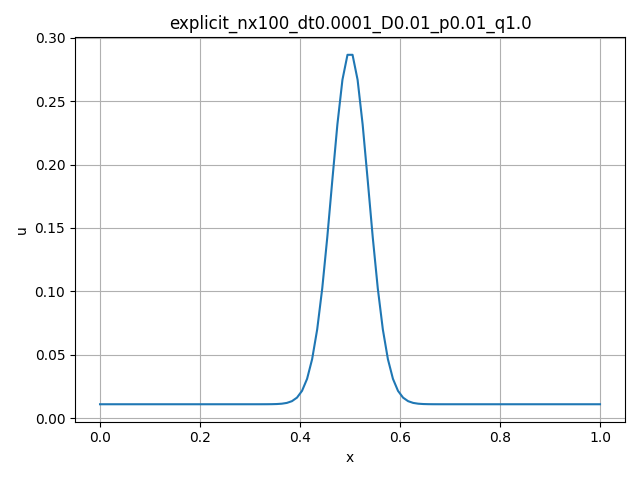
\includegraphics[width=\textwidth]{../zad2/results/explicit_nx100_dt0.0001_D0.01_p0.01_q1.0.png}
    \caption{explicit, nx=100}
  \end{subfigure}\hfill
  \begin{subfigure}[b]{0.4\textwidth}
  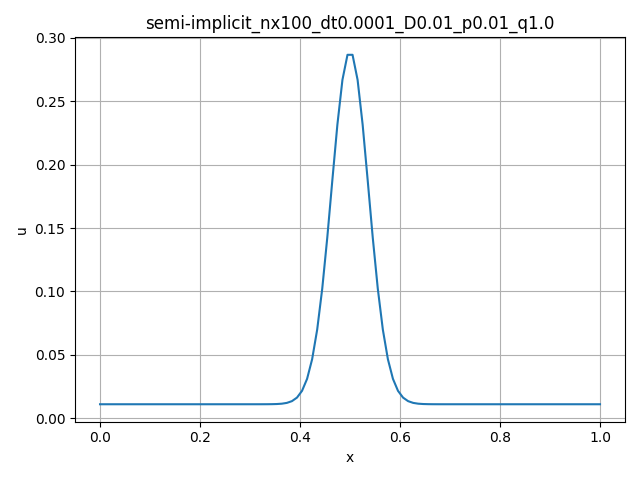
\includegraphics[width=\textwidth]{../zad2/results/semi-implicit_nx100_dt0.0001_D0.01_p0.01_q1.0.png}
    \caption{semi-implicit, nx=100}
  \end{subfigure}
  \vspace{0.5em}
  \begin{subfigure}[b]{0.4\textwidth}
  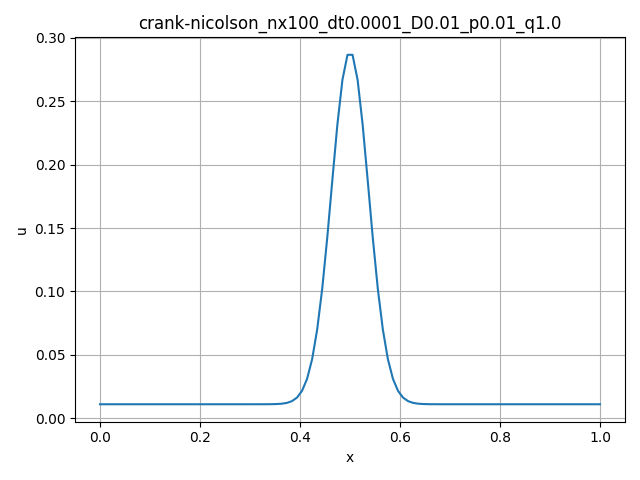
\includegraphics[width=\textwidth]{../zad2/results/crank-nicolson_nx100_dt0.0001_D0.01_p0.01_q1.0.png}
    \caption{Crank--Nicolson, nx=100}
  \end{subfigure}
  \caption{Example profiles $u(x)$ after time $T=0.05$ for one parameter combination (D=0.01,p=0.01,q=1.0).}
\end{figure}
\end{frame}

\begin{frame}{Conclusions}
\begin{itemize}
  \item (1) Computation time: for short tests the explicit solver was fastest due to the low cost of a single step; schemes solving linear systems were slower.
  \item (2) Stability: the explicit solver requires a smaller time step $\Delta t$ as $D$ increases (CFL \(\sim\) $\mathrm{dx}^2/D$); semi-implicit and CN schemes are more robust but more expensive.
  \item (3) Parameters $p,q$: larger $q$ accelerates saturation and may lead to fast local growth; we recommend calibration tests on empirical data.
  \item (4) Parameter ranges (exemplary): for stable simulations at $nx=100$ and $dt=10^{-4}$ sample limits are: $D\lesssim0.1$ (for explicit), $p\in[10^{-4},0.1]$, $q\in[0.1,10]$ - however final limits require a detailed stability and accuracy study.
\end{itemize}
\end{frame}

% --- Task 3 ---
\section*{Task 3 - ODE Surrogate Model for Innovation Diffusion}

\begin{frame}{Introduction to the Surrogate Model}
\begin{itemize}
  \item \textbf{Goal:} Simplify the PDE model to an ODE model by eliminating the spatial variable. This enables much faster simulations.
  \item \textbf{Method:} Averaging the PDE over the whole spatial domain $x \in [0, 1]$.
  $$ \frac{d}{dt} \int_0^1 u(x,t) dx = \int_0^1 D u_{xx} dx + \int_0^1 (p+qu)(1-u) dx $$
  \item With Neumann boundary conditions, the diffusion term vanishes: $\int_0^1 D u_{xx} dx = D[u_x]_0^1 = 0$.
  \item Defining $U(t) = \mathbb{E}[u(x,t)] = \int_0^1 u(x,t) dx$ and applying the approximation $\mathbb{E}[R(u)] \approx R(\mathbb{E}[u])$, we obtain the ODE surrogate model:
  $$ \frac{dU}{dt} = (p + qU)(1-U) $$
\end{itemize}
\end{frame}

\begin{frame}{Neural Network as a Surrogate Model}
\begin{itemize}
    \item \textbf{Goal:} Create a universal surrogate model that generalizes the dynamics for different parameters $D, p, q$.
    \item \textbf{Training data:} A set of PDE simulations for random parameter combinations (learning on many runs).
    \item \textbf{Architecture:} An MLP with a 4-dimensional input $(t, D, p, q)$, two hidden layers and output $U(t)$.
    \item \textbf{Result:} The network learned to map the parameter influence onto the adoption curve, enabling instant prediction for new, previously unseen parameters.
\end{itemize}
\end{frame}

\begin{frame}{Comparison of All Three Models}
\begin{figure}
  \centering
  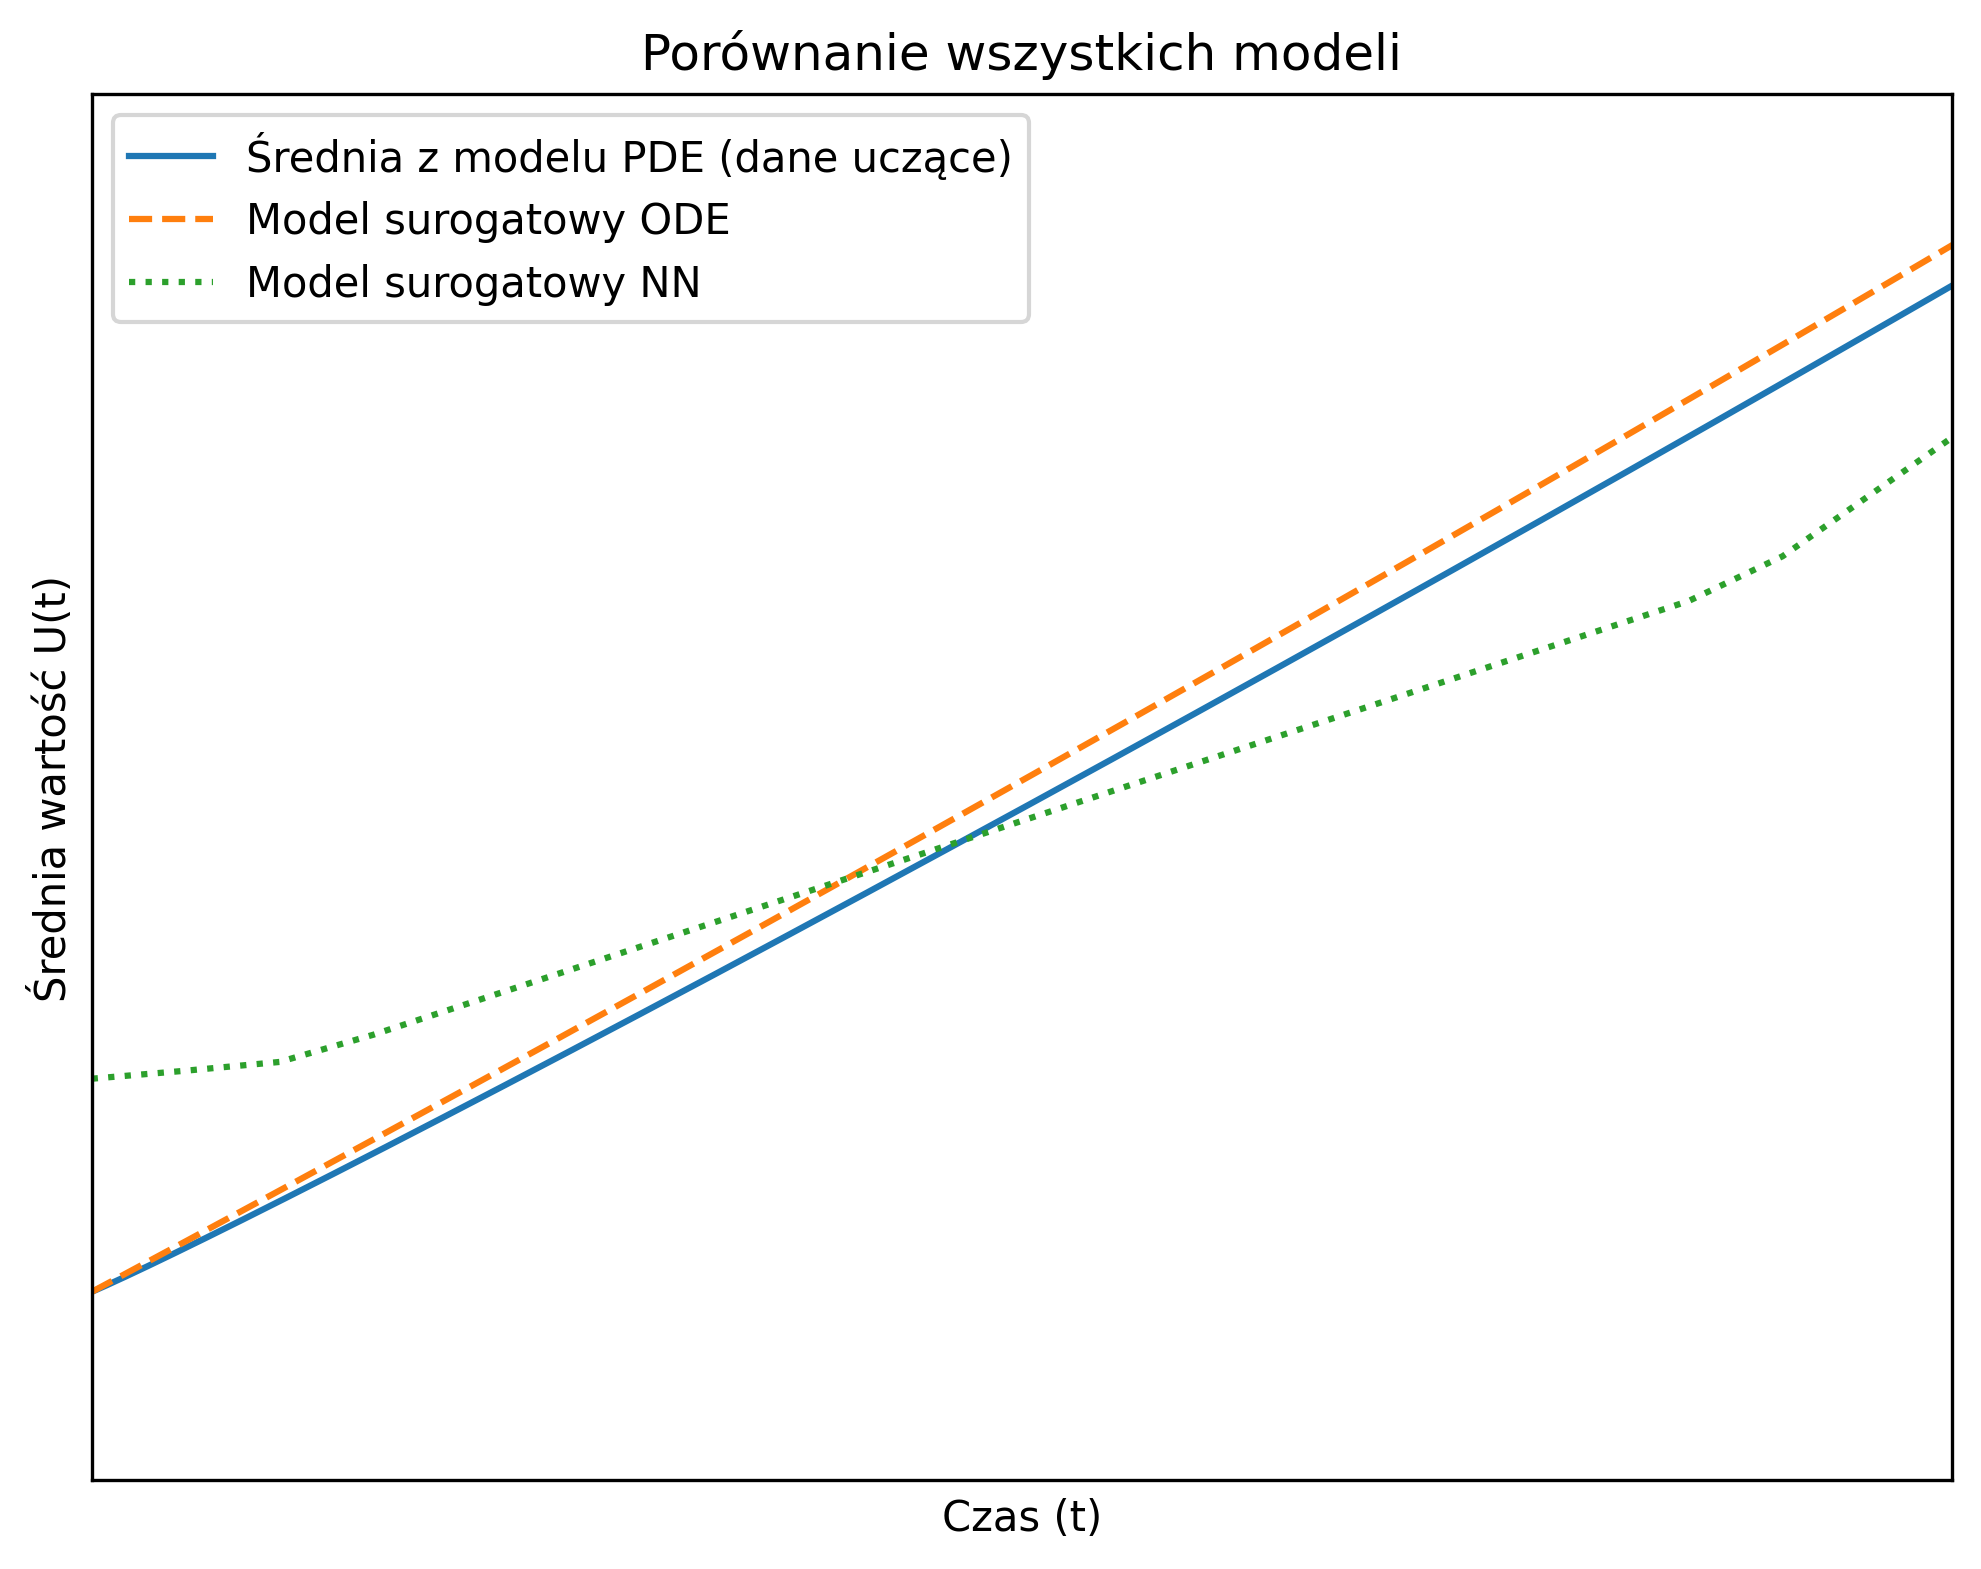
\includegraphics[width=0.7\textwidth]{comparison_plot.png}
  \caption{Comparison of the PDE spatial mean, the ODE surrogate model and the neural network prediction.}
\end{figure}
\begin{itemize}
    \item Test parameters: $D=0.02, p=0.079, q=6.68$.
    \item Inference time for the ODE model: $\approx 0.60$ ms.
    \item Inference time for the NN model: $\approx 0.16$ ms.
\end{itemize}
\end{frame}

\begin{frame}{Final Conclusions}
\begin{itemize}
    \item Surrogate models (both analytic ODE and neural networks) are a powerful tool for accelerating simulations of complex PDE systems.
    \item The ODE model, despite its simplicity, provides a good approximation of the overall system dynamics.
    \item A neural network trained on a set of simulations can generalize and predict dynamics for new parameters with very high accuracy in under 1 ms.
    \item The choice of surrogate model depends on accuracy requirements, data availability and the need for interpretability.
\end{itemize}
\end{frame}

% --- Task 4 ----
\section{Task 4: Sensitivity Analysis}

\begin{frame}{Goal and Methodology of Sensitivity Analysis}
    \begin{itemize}
        \item \textbf{Goal:} Identify which input parameters ($D, p, q$) have the greatest impact on the model output (mean value $U$ at time $t=5.0$).
        \item \textbf{Analyzed models:}
        \begin{itemize}
            \item Full spatio-temporal model (PDE).
            \item Simplified temporal model (ODE surrogate).
        \end{itemize}
        \item \textbf{Methods used:}
        \begin{itemize}
            \item \textbf{Morris method:} Fast screening method for identifying the most important parameters. Measures overall influence ($\mu^*$) and interactions/nonlinearity ($\sigma$).
            \item \textbf{Sobol method:} Global variance-based method. More accurate but more expensive. Decomposes output variance into individual parameter contributions ($S1$) and interactions ($ST$).
        \end{itemize}
    \end{itemize}
\end{frame}

\begin{frame}{Results - Morris Method}
    \begin{columns}[T]
        \begin{column}{0.5\textwidth}
            \centering
            \textbf{ODE model}\\
            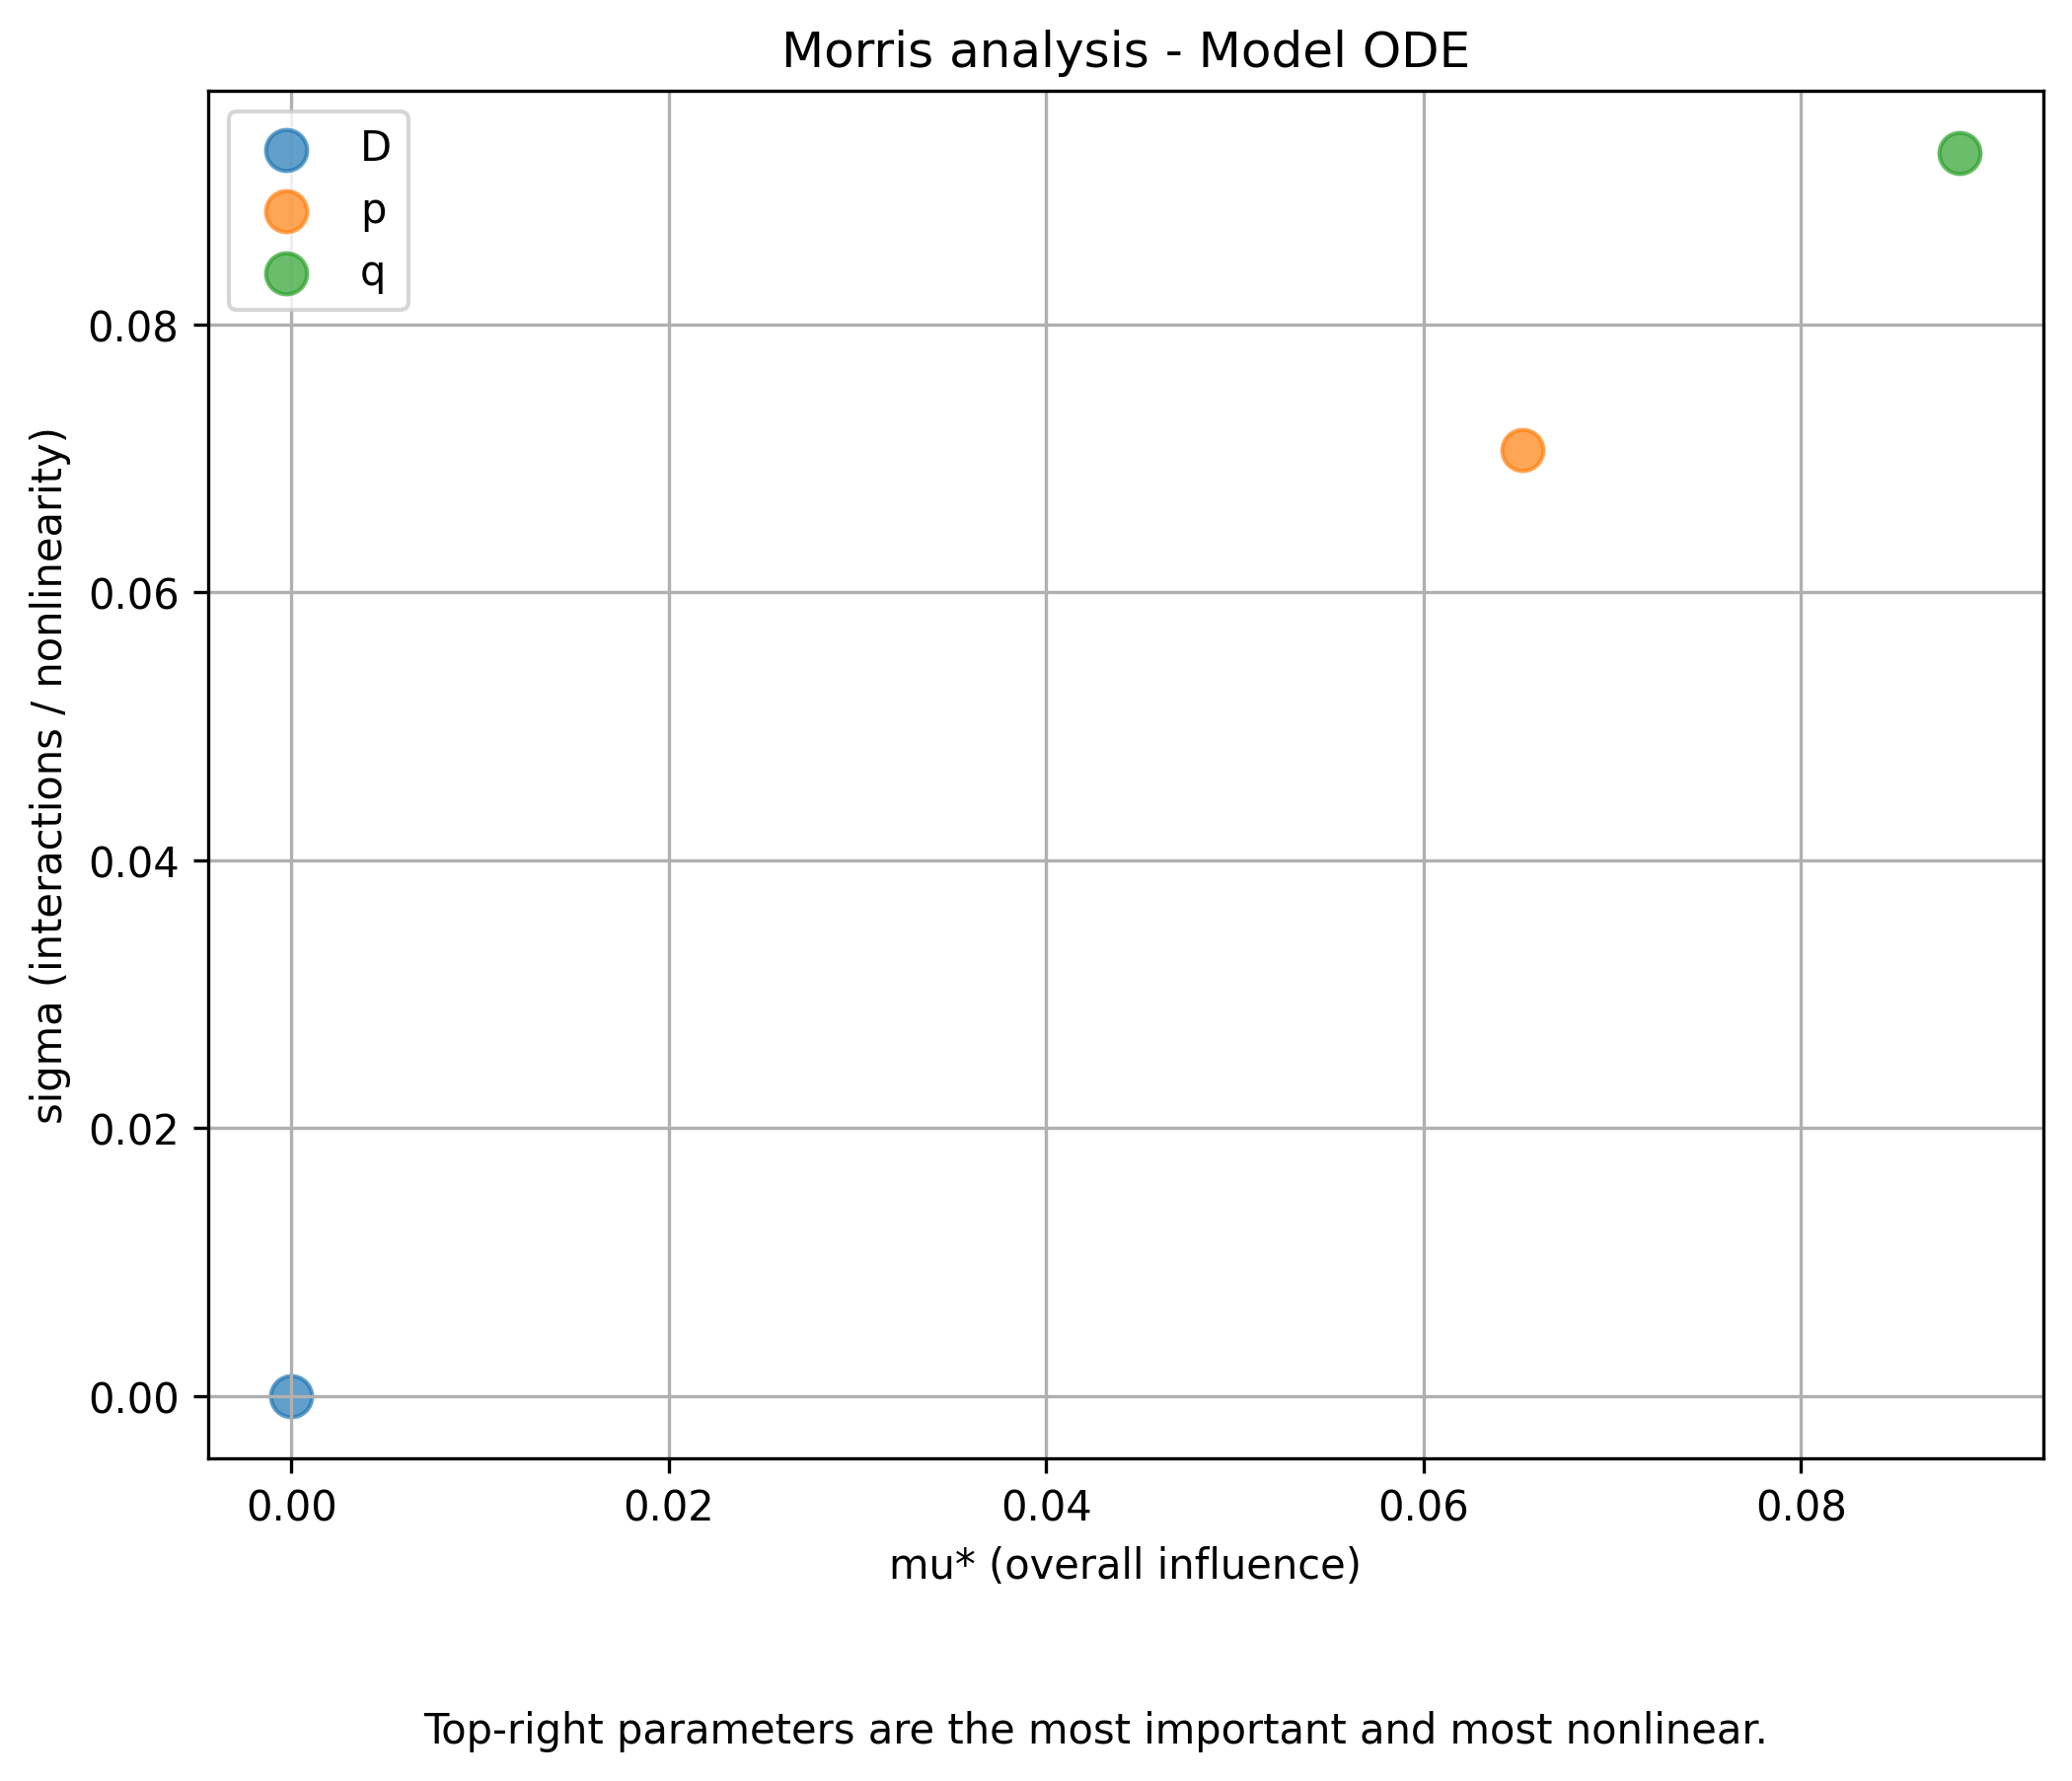
\includegraphics[width=\textwidth]{figures/morris_model_ode.png}
        \end{column}
        \begin{column}{0.5\textwidth}
            \centering
            \textbf{PDE model}\\
            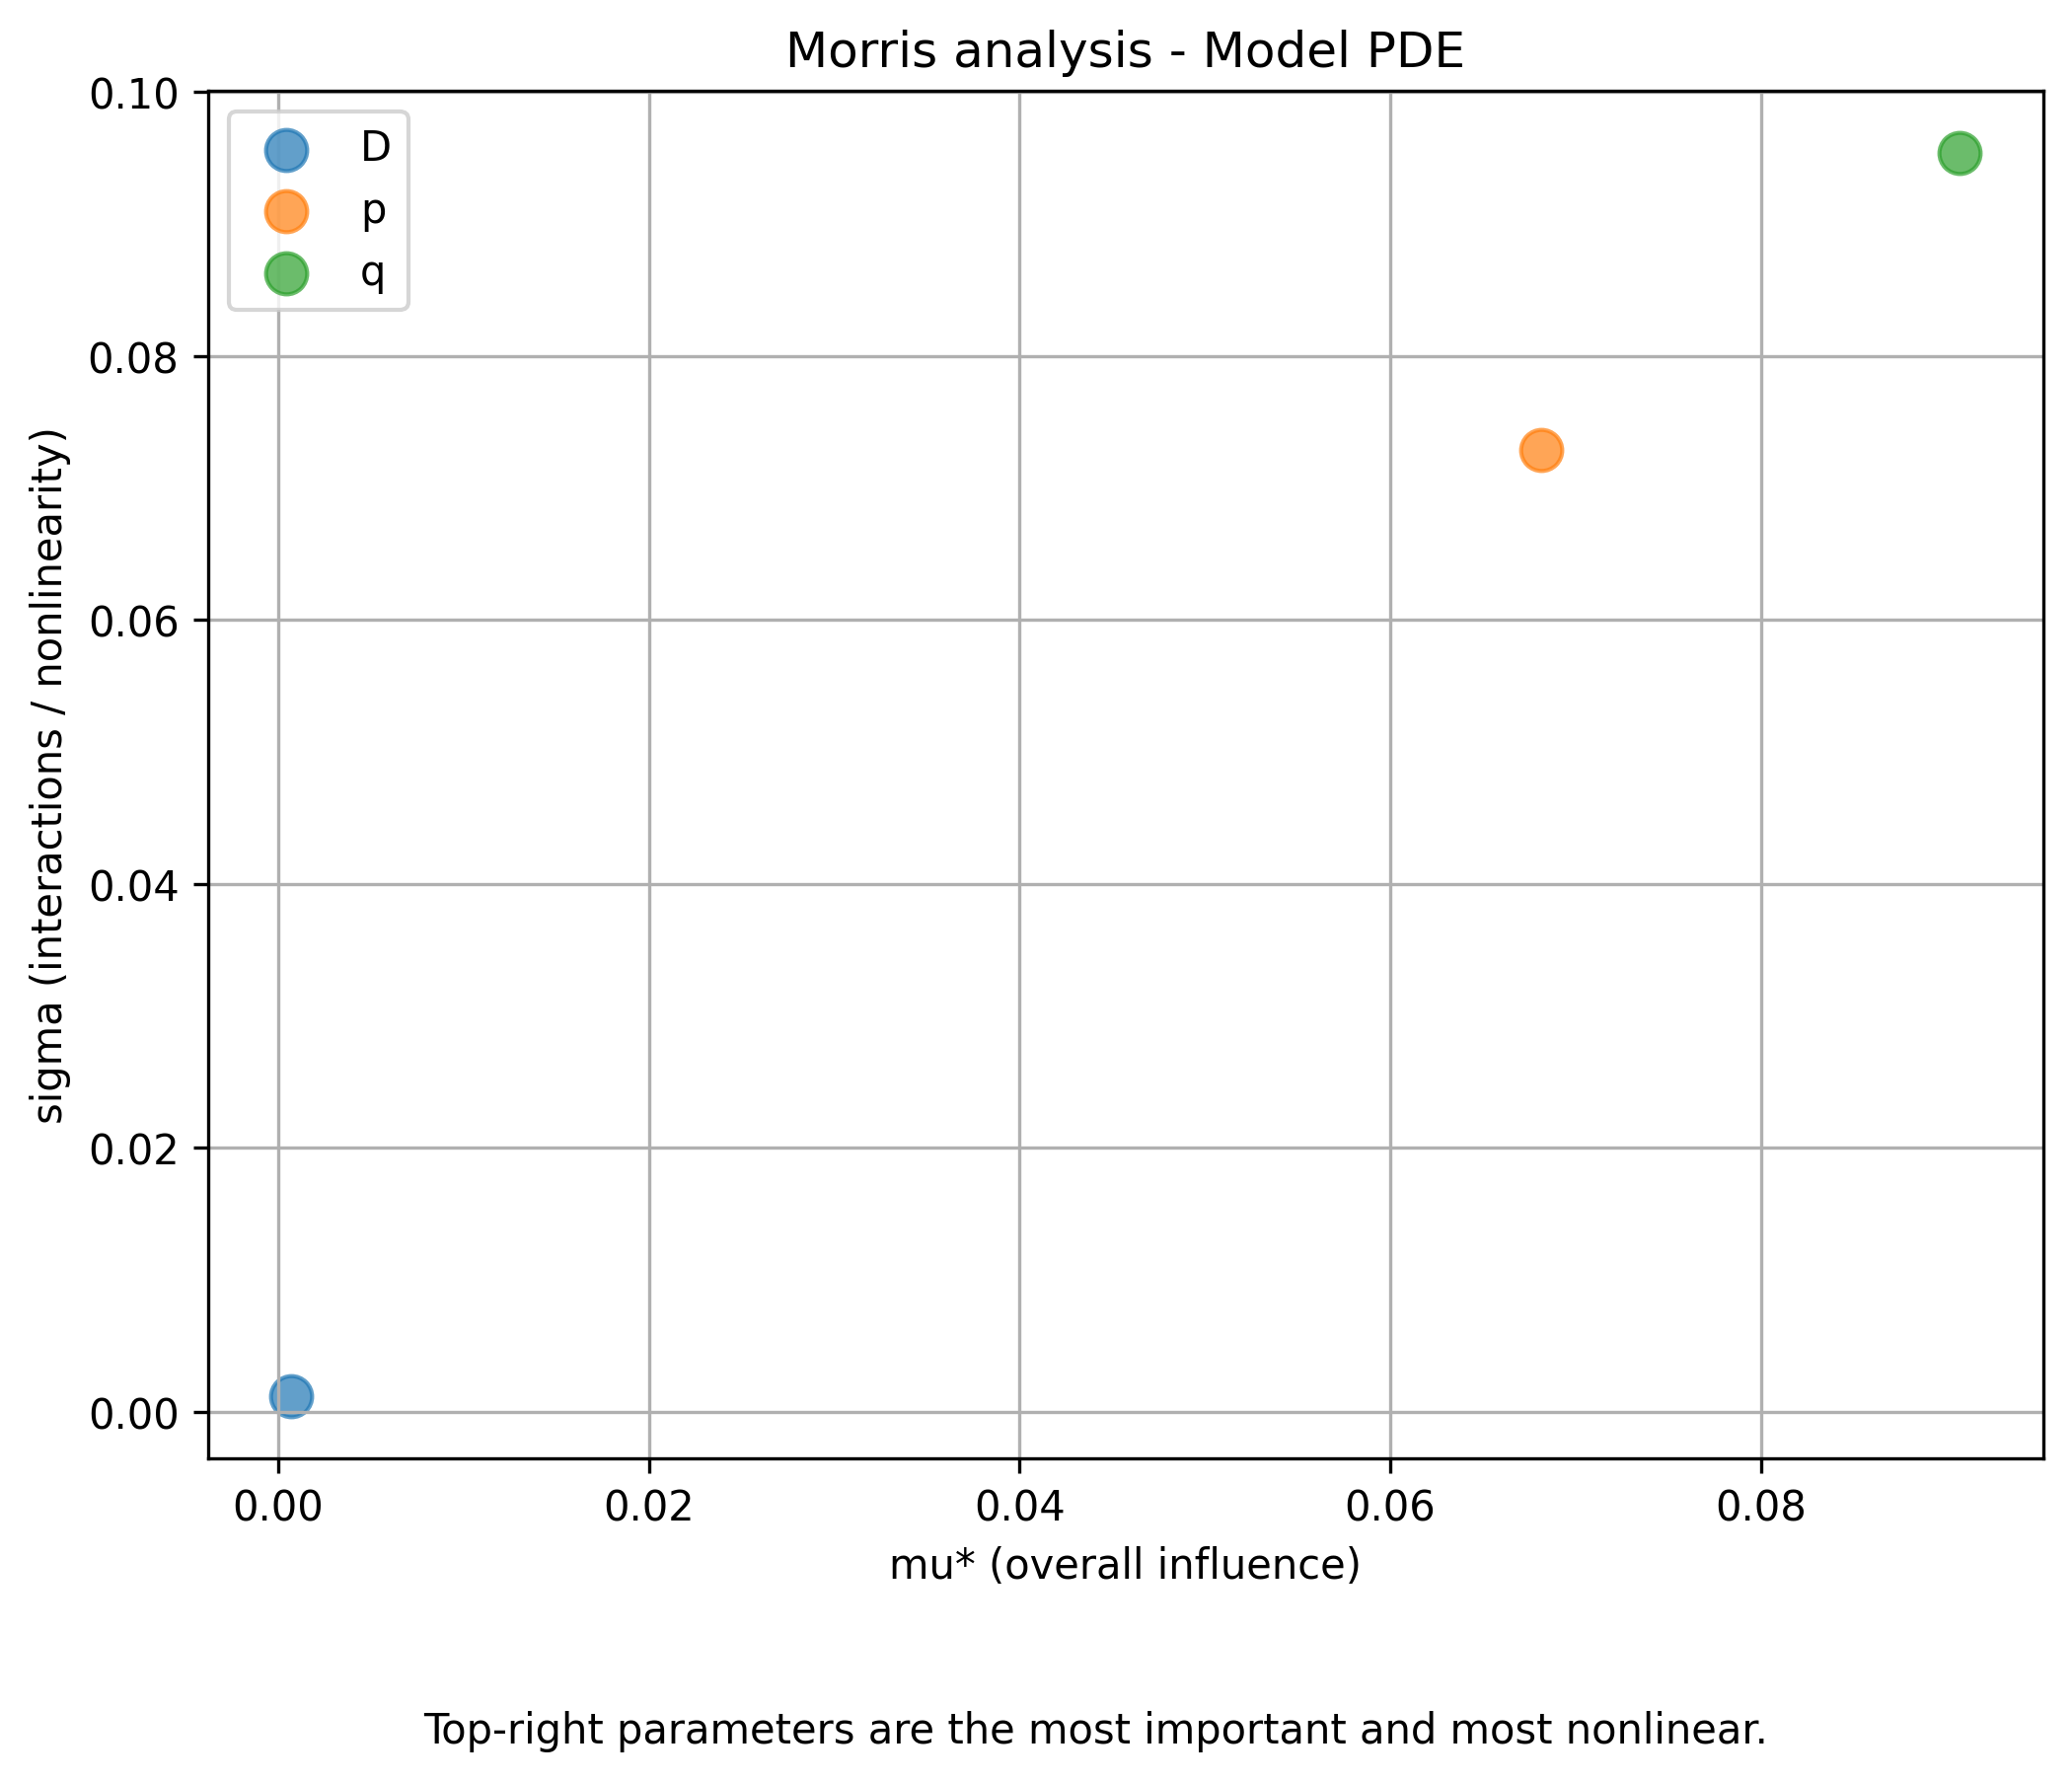
\includegraphics[width=\textwidth]{figures/morris_model_pde.png}
        \end{column}
    \end{columns}
    \begin{itemize}
        \item \textbf{Conclusions:} In both models, parameter \textbf{q} (imitation) shows the greatest influence (highest $\mu^*$) and significant interactions (high $\sigma$). Parameter \textbf{p} has a moderate influence, and \textbf{D} (in the PDE model) is the least important.
    \end{itemize}
\end{frame}

\begin{frame}{Results - Sobol Method}
    \begin{columns}[T]
        \begin{column}{0.5\textwidth}
            \centering
            \textbf{ODE model}\\
            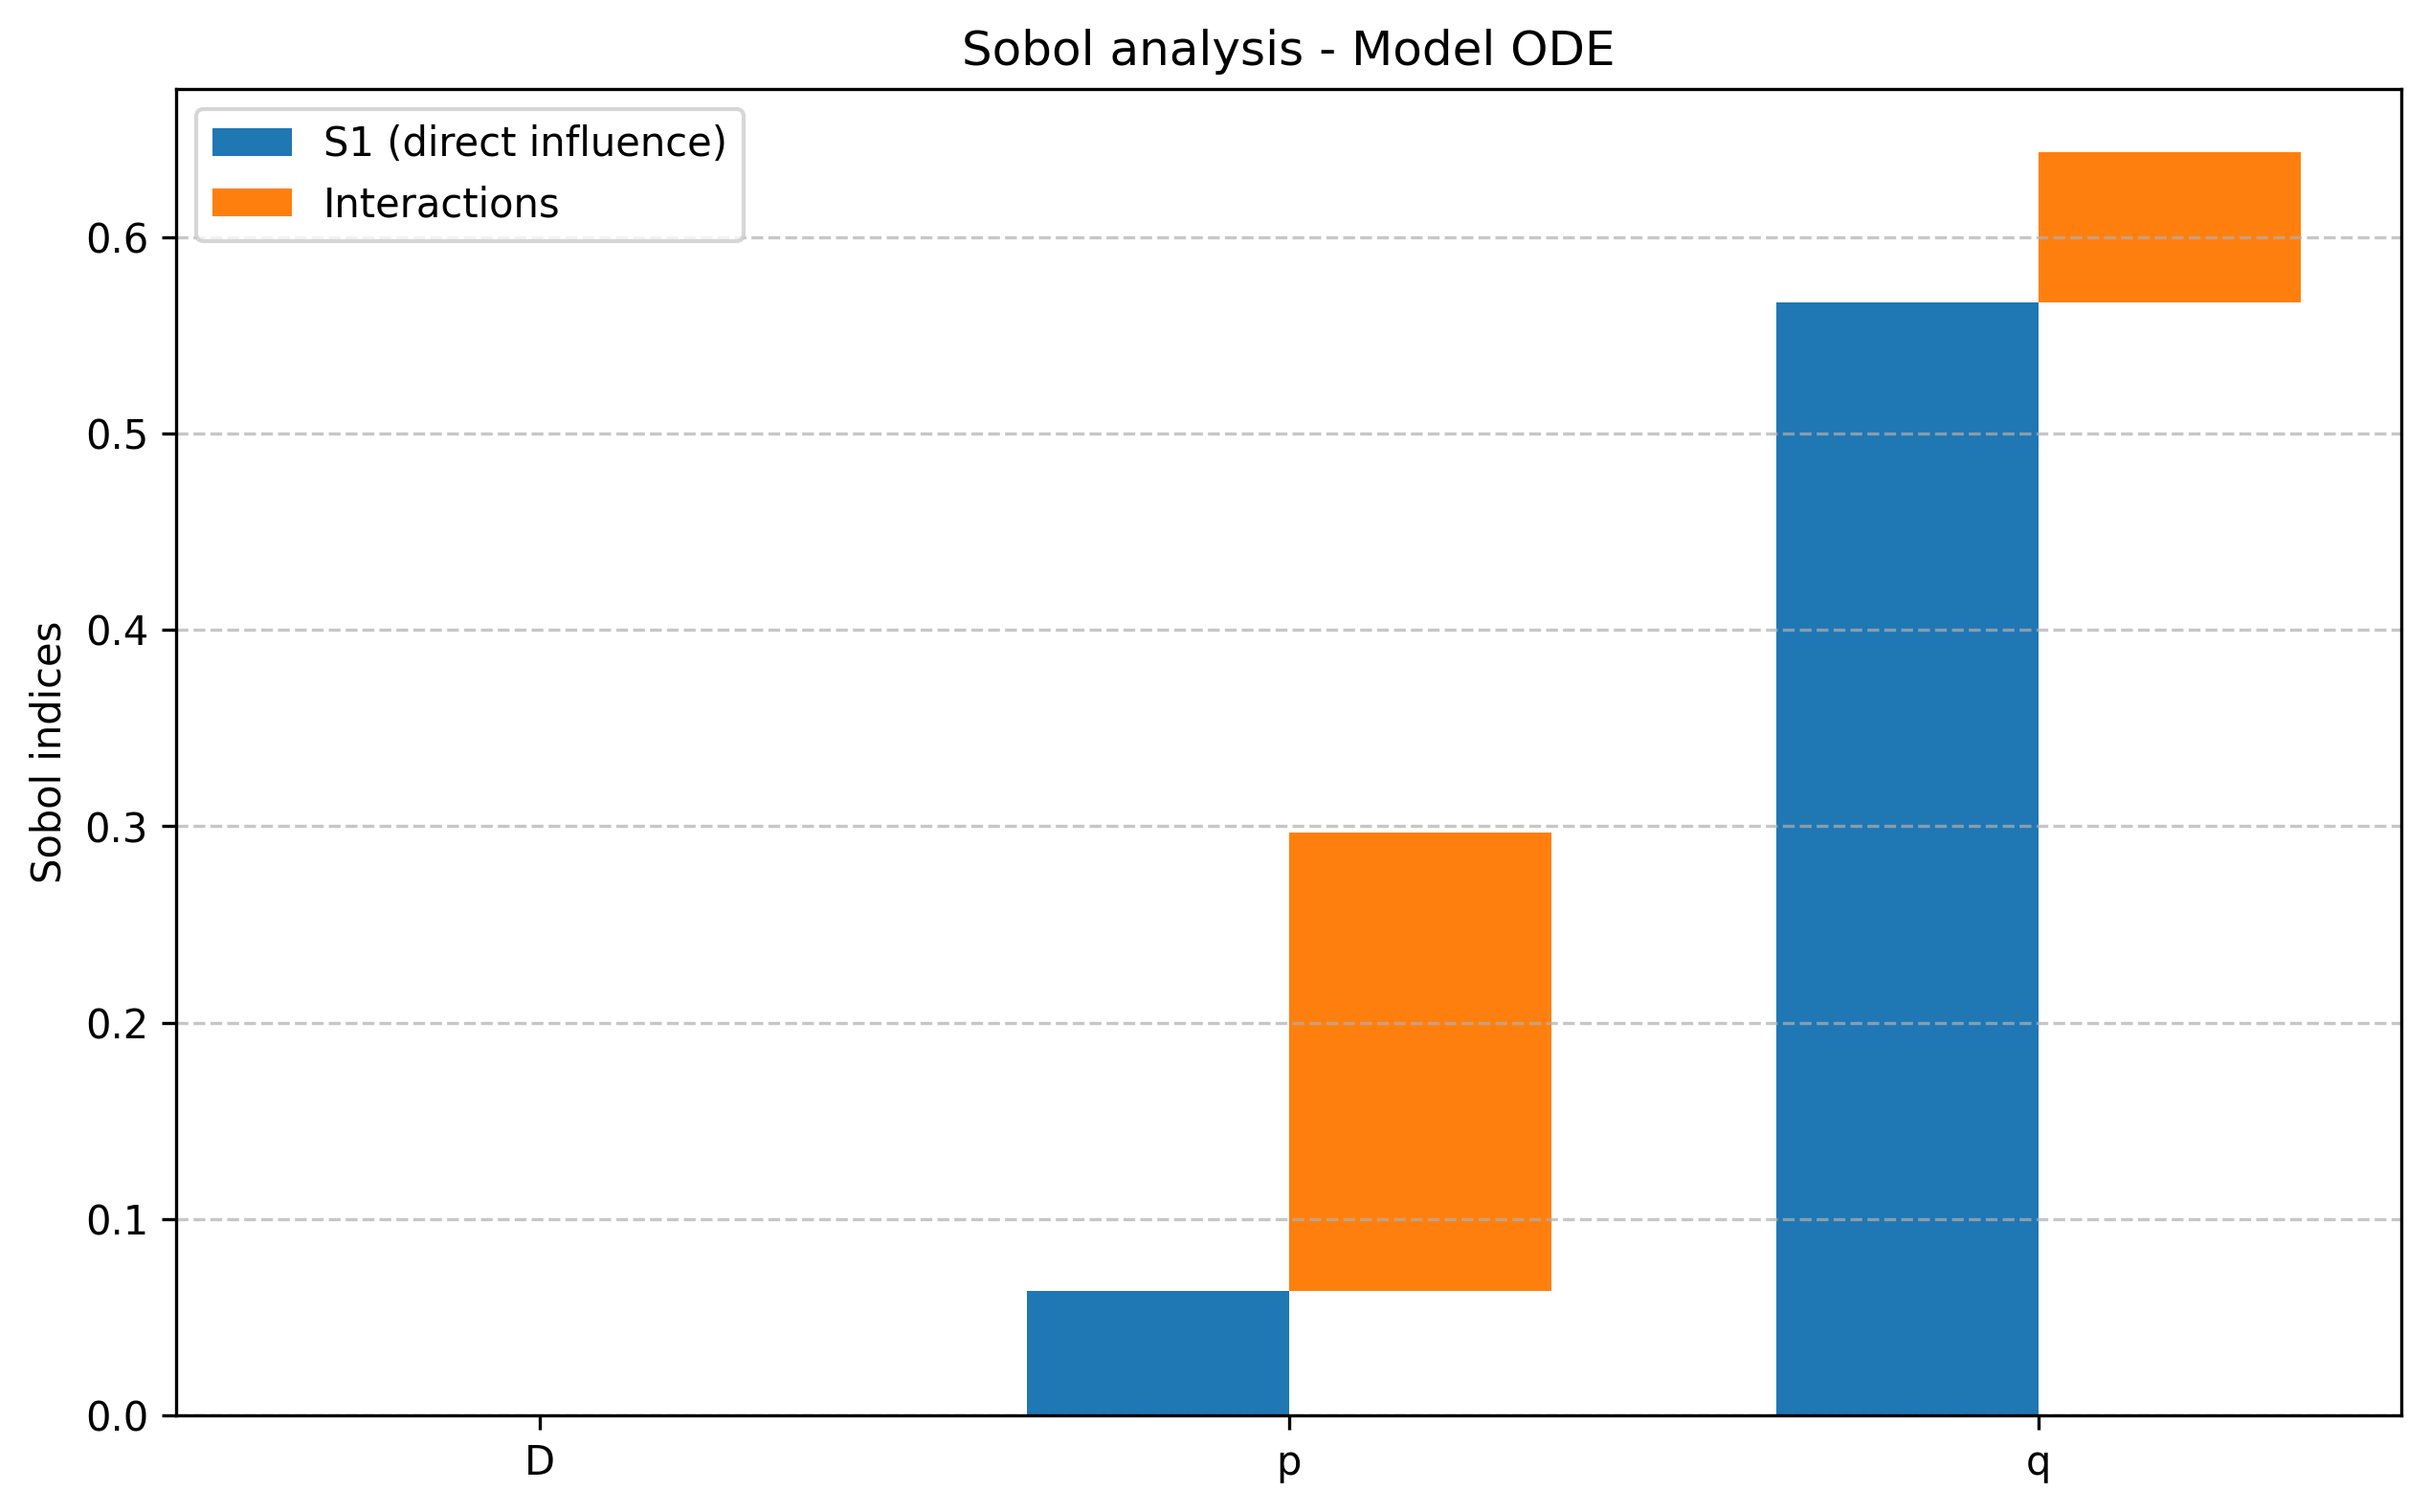
\includegraphics[width=\textwidth]{figures/sobol_model_ode.png}
        \end{column}
        \begin{column}{0.5\textwidth}
            \centering
            \textbf{PDE model}\\
            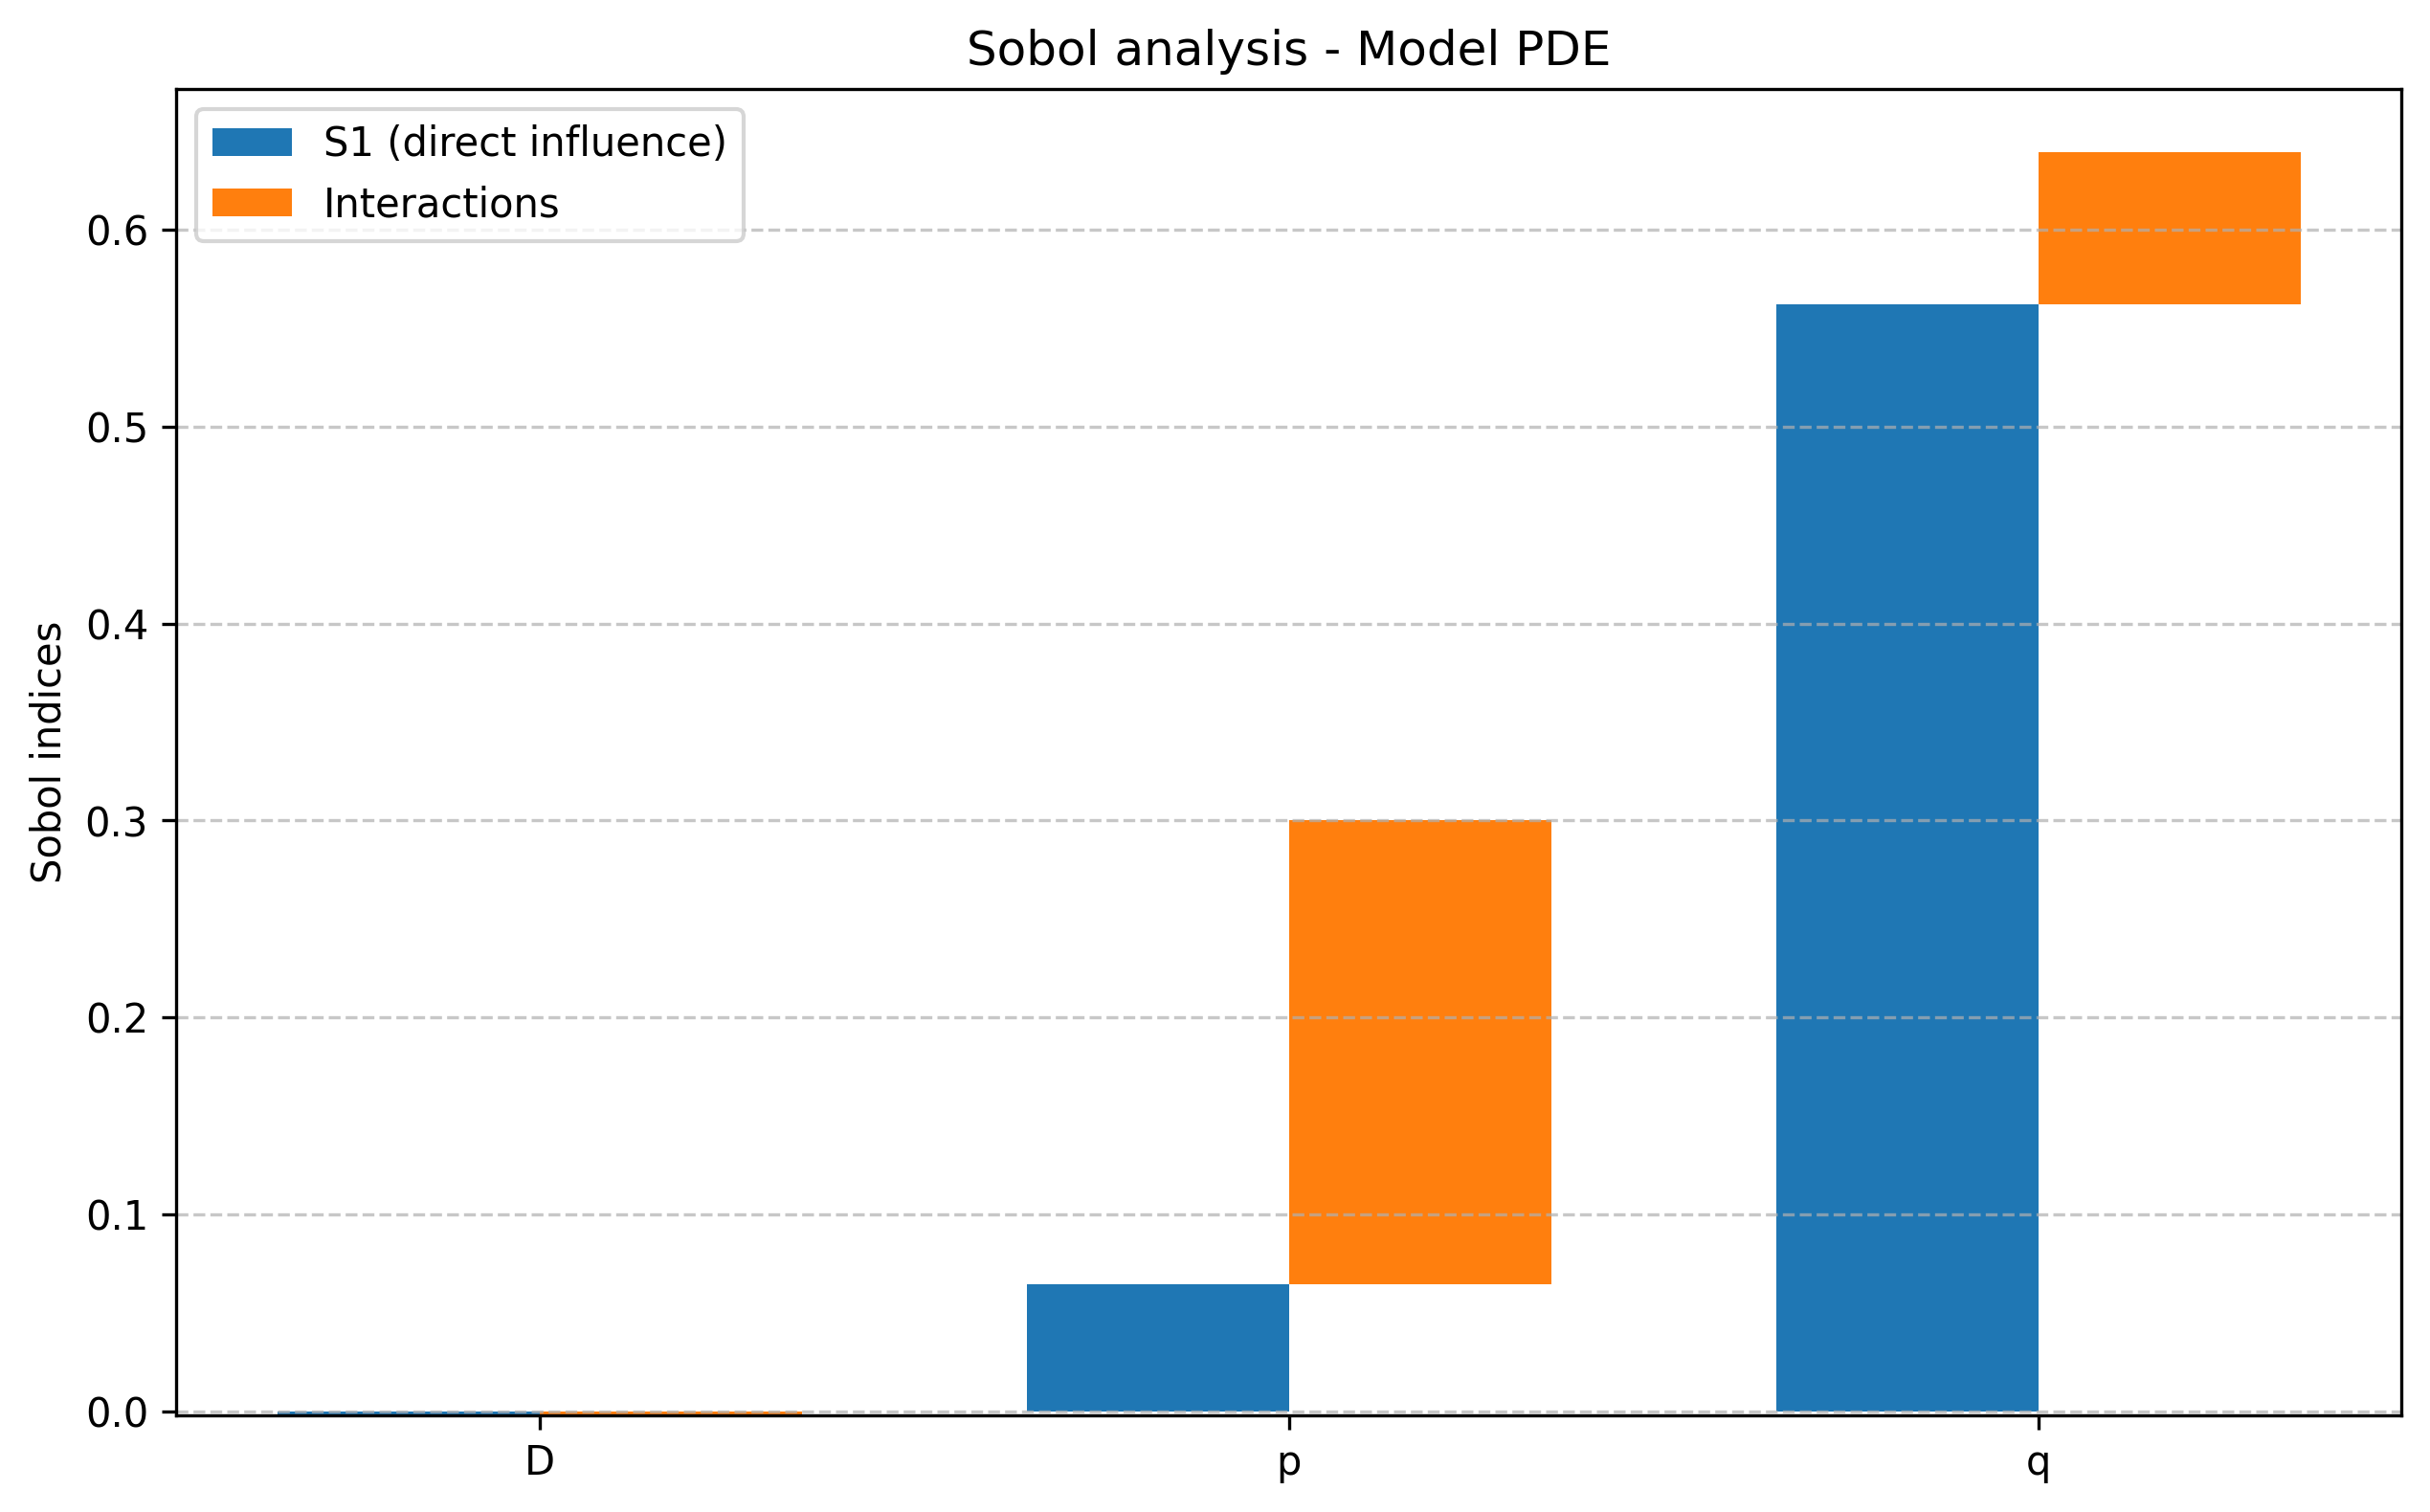
\includegraphics[width=\textwidth]{figures/sobol_model_pde.png}
        \end{column}
    \end{columns}
    \begin{itemize}
        \item \textbf{Confirmation:} Sobol analysis confirms the Morris results.
        \item \textbf{Total influence (ST):} Parameter \textbf{q} has the dominant influence.
        \item \textbf{Interactions:} The large difference between $ST$ and $S1$ for parameter $q$ indicates strong interactions with other parameters.
        \item \textbf{Influence of D:} The influence of parameter $D$ on the mean value $U(t)$ is marginal.
    \end{itemize}
\end{frame}

\begin{frame}{Conclusions and Model Simplification}
    \textbf{Conclusions from sensitivity analysis:}
    \begin{itemize}
        \item The imitation parameter ($q$) is the key factor controlling the dynamics of the mean adoption level $U(t)$.
        \item The innovation parameter ($p$) is secondary but still significant.
        \item The diffusion parameter ($D$) has negligible influence on the \textit{mean} value of the system, although it is crucial for the \textit{spatial} dynamics.
    \end{itemize}
    \vspace{1cm}
    \textbf{Proposed model simplification:}
    \begin{itemize}
        \item The ODE model is already a simplification that ignores $D$. The analysis confirms this is justified if only the mean value $U(t)$ matters.
        \item In the PDE model, parameter $D$ could be fixed at a constant value (e.g. its mean over the studied range) without much accuracy loss for this particular output measure. This reduces the problem complexity by one dimension.
    \end{itemize}
\end{frame}

% --- Task 5 ---
\section*{Task 5 - Data Assimilation (ABC and 3D-Var)}

\begin{frame}{Data Assimilation Problem Formulation}
\begin{itemize}
  \item \textbf{Goal:} Reconstruct the model parameters and system state from noisy observations within a time window.
  \item \textbf{Methods:}
    \begin{itemize}
      \item \textbf{ABC (Approximate Bayesian Computation):} A gradient-free method based on sampling parameters and accepting those that generate results close to the observations. Robust to local minima but computationally expensive.
      \item \textbf{3D-Var (Variational):} Minimization of the cost function $J(x) = ||y - H(x)||^2$. Fast convergence when gradients are available, but risks getting stuck in local minima.
    \end{itemize}
  \item \textbf{Experiment:} "Real" data from the PDE model + Gaussian noise. Tests for the ODE surrogate and the full PDE with three time budgets (Low: 2s, Medium: 5s, High: 15s).
\end{itemize}
\end{frame}

\begin{frame}{Assimilation Results for the ODE Model}
\begin{columns}
\column{0.5\textwidth}
\begin{itemize}
  \item \textbf{3D-Var:} Very fast convergence (time < 0.1s). Minimal RMSE ($\approx 0.006$). The ideal method for the simple ODE model.
  \item \textbf{ABC:} Requires many iterations (thousands). Stable error ($\approx 0.012$), but higher than 3D-Var.
  \item \textbf{Conclusions:} For cheap numerical models, gradient-based (or quasi-Newton) methods are unbeatable.
\end{itemize}
\column{0.5\textwidth}
\begin{figure}
  \centering
  
\includegraphics[width=\textwidth]{../zad5/results/ode_assimilation_results_budget_high.png}
  \caption{ODE assimilation results (High budget). The red line (Var) matches the truth almost perfectly.}
\end{figure}
\end{columns}
\end{frame}

\begin{frame}{Assimilation Results for the PDE Model}
\begin{columns}
\column{0.5\textwidth}
\begin{itemize}
  \item \textbf{Challenge:} A single PDE evaluation is costly, which limits the number of iterations within a budget.
  \item \textbf{ABC:} Reaches an approximate solution with RMSE $\approx 0.027$ - stable but clearly suboptimal.
  \item \textbf{3D-Var:} After reusing the sparse factorization in the PDE solve (5x fewer iterations needed per evaluation), the optimizer converges to RMSE $\approx 0.002$ - an order of magnitude better than ABC.
\end{itemize}
\column{0.5\textwidth}
\begin{figure}
  \centering
  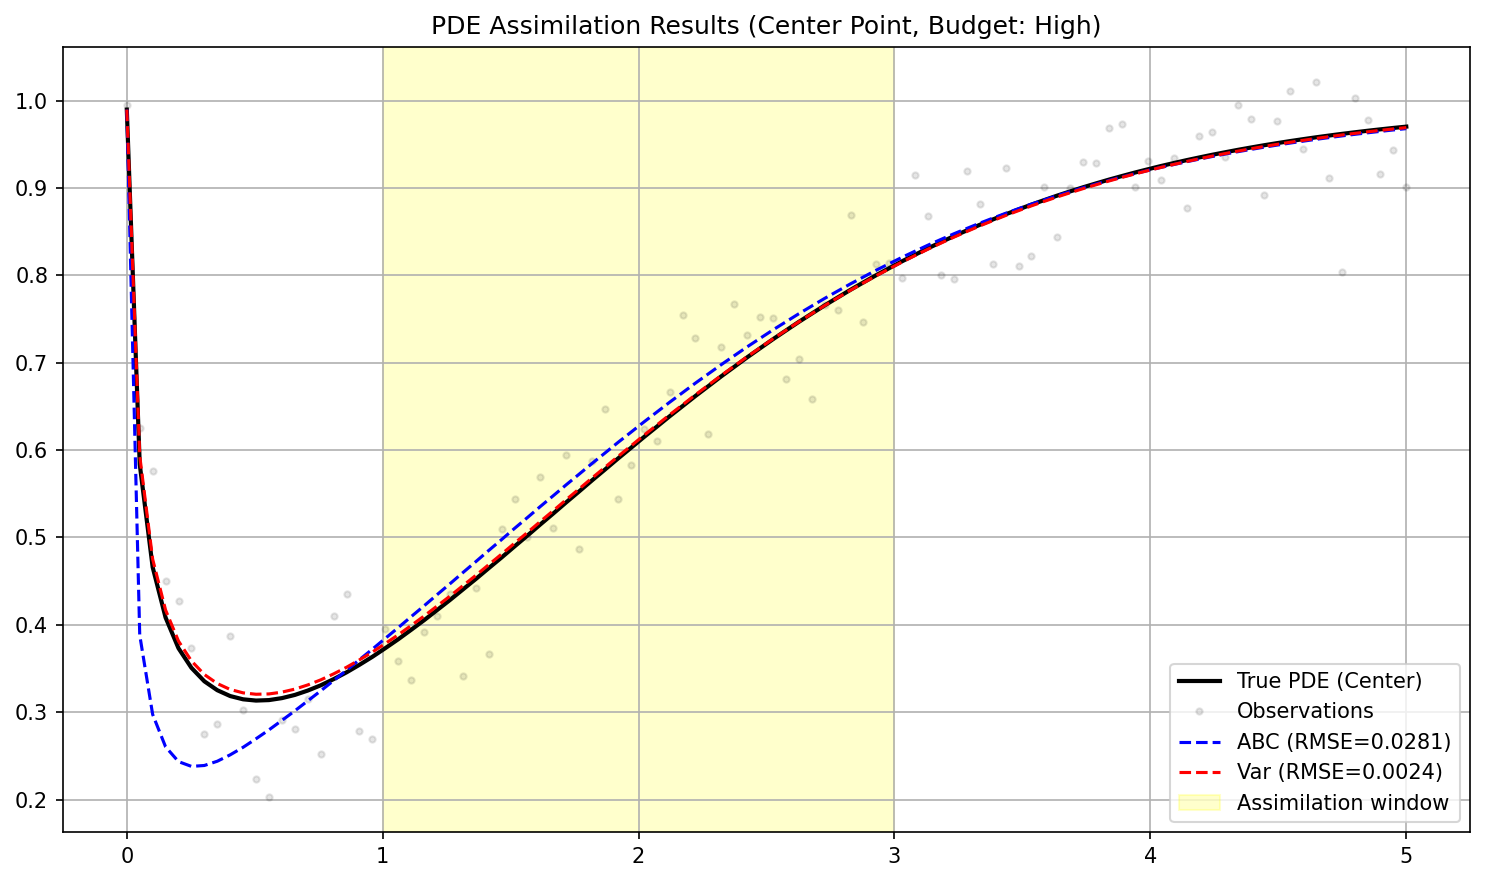
\includegraphics[width=\textwidth]{../zad5/results/pde_assimilation_results_center_budget_high.png}
  \caption{PDE assimilation results (High budget). Var (red) matches the truth almost perfectly.}
\end{figure}
\end{columns}
\end{frame}

\begin{frame}{Summary of Results (RMSE)}
\begin{table}
\centering
\begin{tabular}{l|l|c|c|c}
\textbf{Model} & \textbf{Method} & \textbf{Low (2s)} & \textbf{Medium (5s)} & \textbf{High (15s)} \\
\hline
ODE & ABC & 0.0118 & 0.0116 & 0.0113 \\
ODE & 3D-Var & \textbf{0.0061} & \textbf{0.0061} & \textbf{0.0061} \\
\hline
PDE & ABC & 0.0271 & 0.0291 & 0.0281 \\
PDE & 3D-Var & \textbf{0.0017} & \textbf{0.0024} & \textbf{0.0024} \\
\end{tabular}
\caption{Comparison of trajectory-wide RMSE prediction errors.}
\end{table}
\textbf{Conclusion:} Once the model evaluation is cheap enough (factorized sparse solver), gradient-based variational methods clearly outperform stochastic ABC under the same time budgets.
\end{frame}

% --- Task 6 ---
\section*{Task 6 - PINN (Physics-Informed Neural Network)}

\begin{frame}{PINN Concept}
\begin{itemize}
  \item \textbf{Idea:} Combine observational data with the physical knowledge contained in the differential equations (PDE).
  \item \textbf{Architecture:} A neural network $u_{NN}(x,t)$ approximating the solution.
  \item \textbf{Loss function:} $L = L_{data} + L_{physics}$
    \begin{itemize}
      \item $L_{data} = \frac{1}{N_d} \sum (u_{NN}(x_i, t_i) - u_{obs})^2$ (data fit)
      \item $L_{physics} = \frac{1}{N_f} \sum |f(u_{NN}(x_j, t_j))|^2$ (PDE residual)
    \end{itemize}
  \item \textbf{Advantage:} The ability to train on sparse data and "fill in" the missing information with physics.
\end{itemize}
\end{frame}

\begin{frame}{Implementation and Training Run}
\begin{itemize}
  \item \textbf{Configuration (hardened):} $nx=150$, $\Delta t=5\cdot10^{-4}$, $N_{data}=1200$, $N_{f}=12000$, noise \texttt{gaussian\_mixture} 5\%.
  \item \textbf{Network:} MLP (5 layers $\times$ 64, Tanh) with \textbf{residual connections}; \textbf{epochs:} 2000; \textbf{time:} \(~75.75\,\)s, CPU.
  \item \textbf{Optimization techniques:} Learning rate scheduler (StepLR, $\gamma=0.9$), gradient clipping, \textbf{warmup strategy for the physics weights} ($\lambda_{phy}$: 0.1 $\to$ 2.0 over 500 epochs).
  \item \textbf{Loss (last):} $L \approx 0.006$ (Data $\approx 0.0056$, Physics $\approx 0.00022$) - significant improvement in stability and convergence.
\end{itemize}

\begin{figure}
  \centering
  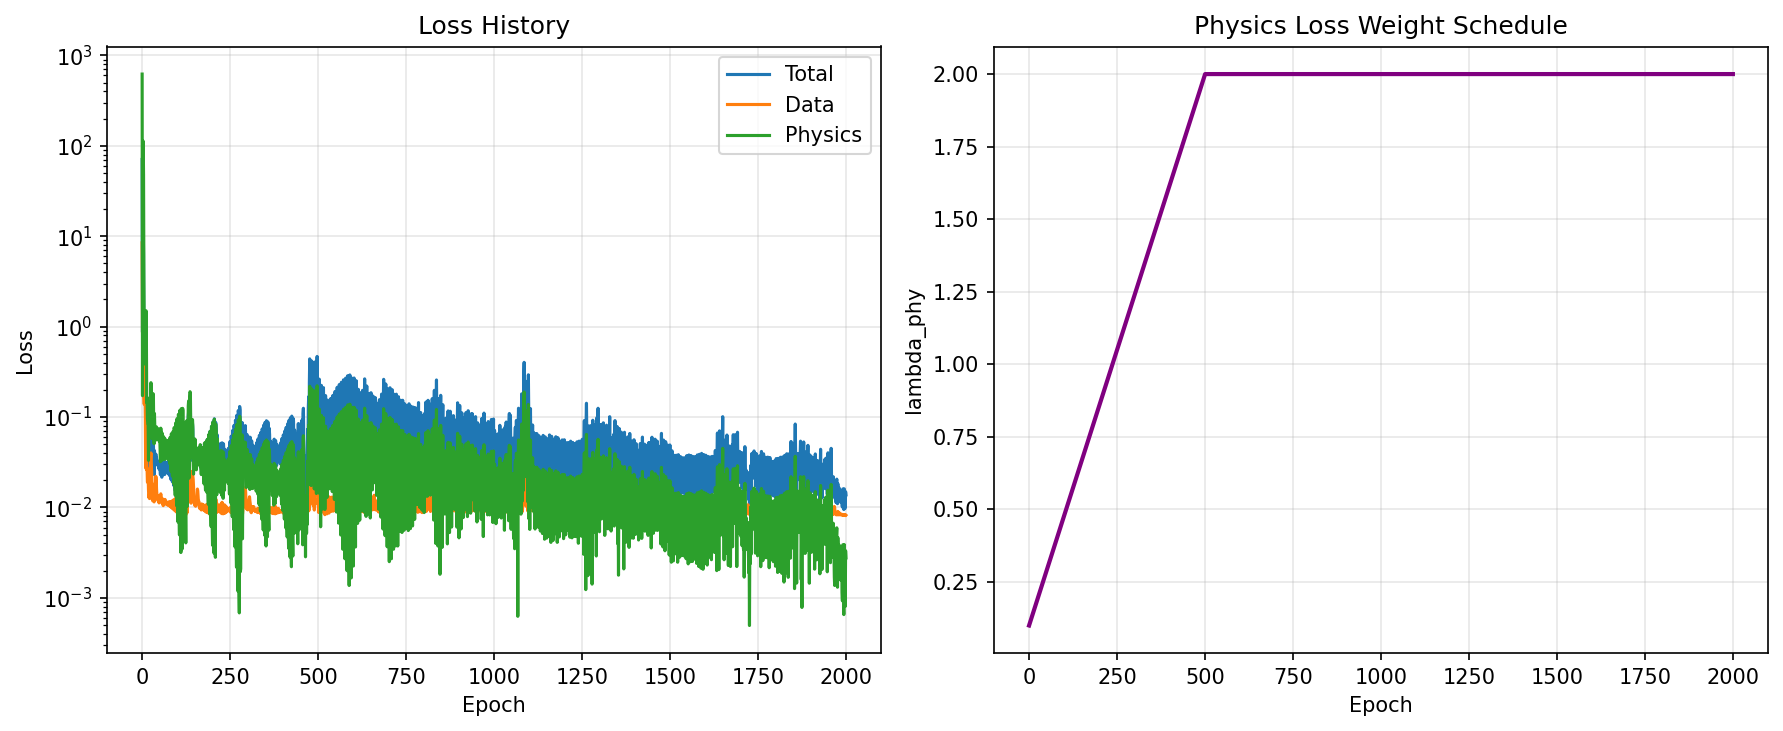
\includegraphics[height=0.4\textheight]{../zad6/results/loss_history_improved.png}
  \caption{Loss history. Smooth convergence thanks to the residual architecture and $\lambda$ warmup.}
\end{figure}

\end{frame}

\begin{frame}{Field Reconstruction Results (PINN vs PDE)}
\begin{figure}
  \centering
  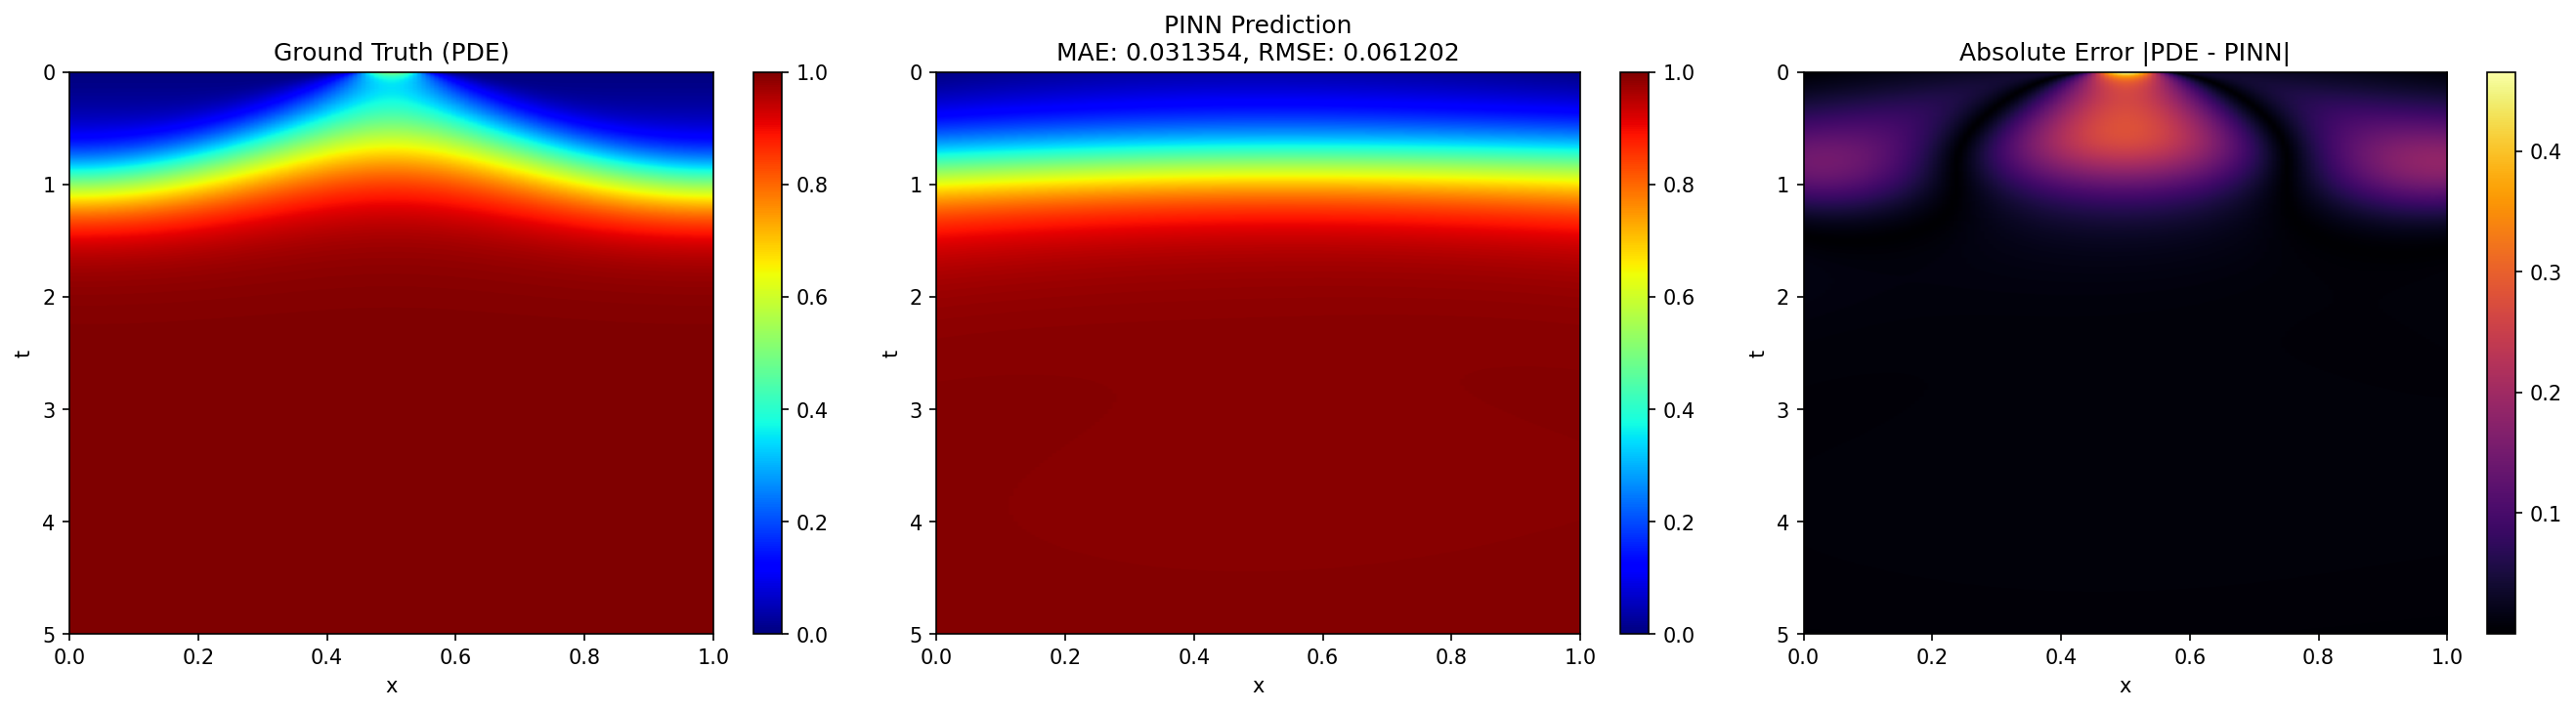
\includegraphics[width=\textwidth]{../zad6/results/pinn_results_heatmap_improved.png}
  \caption{Comparison of the reference solution (PDE), the (improved) PINN prediction and the absolute error. The error is distributed evenly and nearly invisible.}
\end{figure}
\begin{itemize}
    \item \textbf{MAE:} 0.031354 (vs. 0.1855 baseline) --- \textbf{83.1\% reduction} \quad
    \item \textbf{RMSE:} 0.061202 (vs. 0.2359) --- \textbf{74.1\% reduction} \quad
    \item \textbf{relL2:} 0.068676 (vs. 0.2647) --- \textbf{74.1\% reduction}
    \item The residual architecture and warmup strategy enable much better physics learning despite the noise.
\end{itemize}
\end{frame}

\begin{frame}{Mean Dynamics Comparison (PINN vs PDE vs ODE)}
\begin{figure}
  \centering
  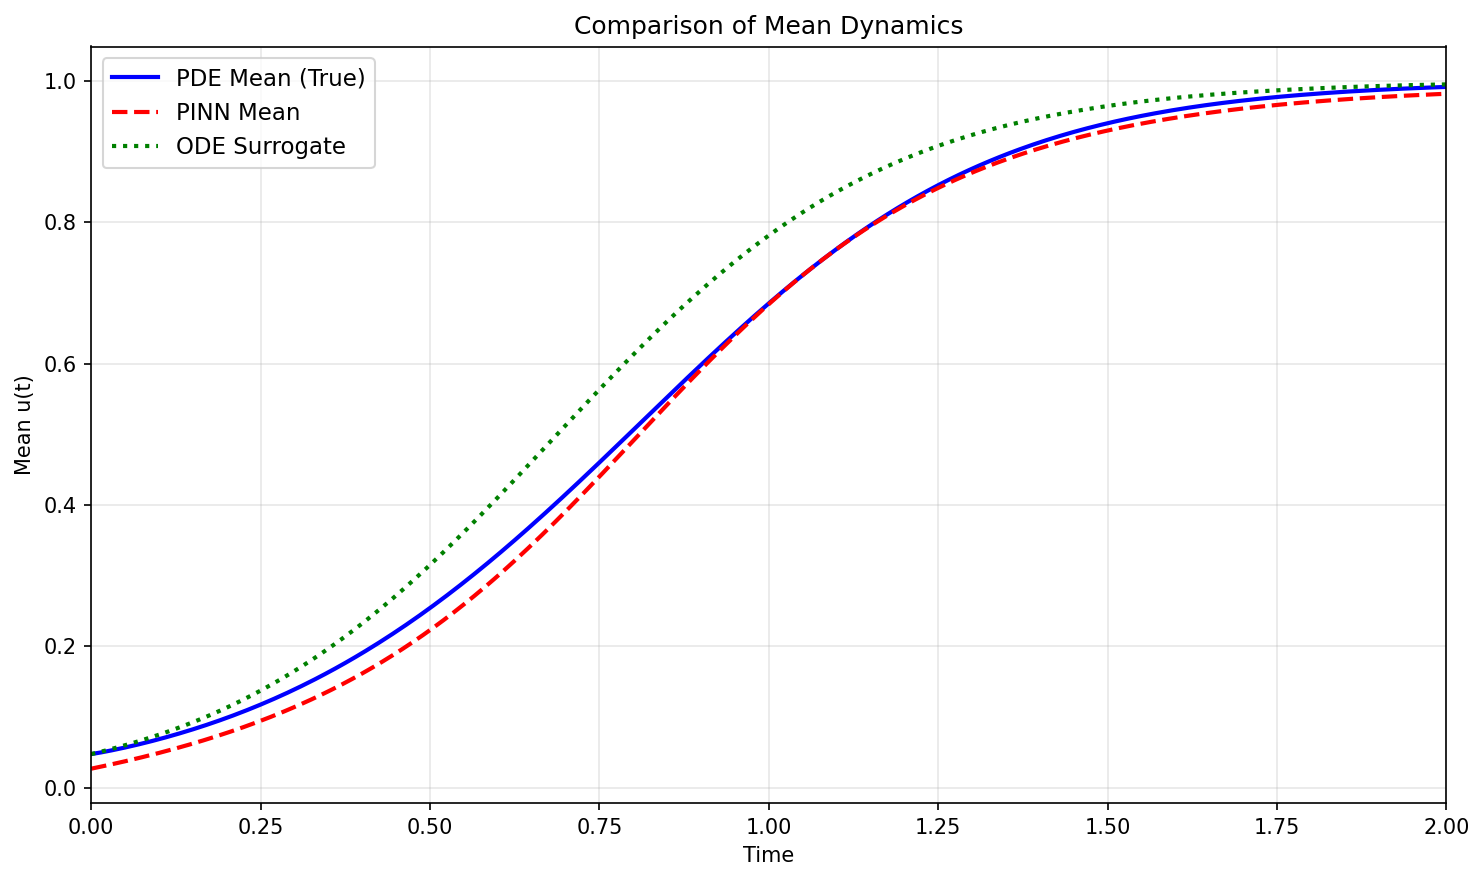
\includegraphics[width=0.8\textwidth]{../zad6/results/pinn_vs_pde_vs_ode_improved.png}
  \caption{Comparison of the spatial mean $u(t)$. The (improved) PINN (red dashed) almost perfectly matches the PDE (black solid).}
\end{figure}
\begin{itemize}
  \item The \textbf{improved PINN} tracks the true PDE trajectory very accurately
  \item Both methods (PINN and ODE surrogate) agree over the whole time window
  \item The improvement results from: (1) a deeper network, (2) residual connections, (3) adaptive physics weighting and (4) better optimization
\end{itemize}
\end{frame}

% --- Task 7 ---
\section*{Task 7 - SuperModel (ODE) and SuperNet (PINN)}

\begin{frame}{The Supermodeling Concept}
\begin{itemize}
  \item \textbf{Problem:} Models often have inaccurate parameters.
  \item \textbf{Solution:} Combine many "imperfect" models into one ensemble that learns a consensus.
  \item \textbf{SuperModel ODE:} An ensemble of ODE models coupled by a relaxation (nudging) term towards the mean trajectory.
  \item \textbf{SuperNet PINN:} An ensemble of neural networks trained in parallel with an additional \textit{Coupling Loss}, enforcing prediction consistency at collocation points.
\end{itemize}
\end{frame}

\begin{frame}{Results: SuperModel ODE}
\begin{figure}
  \centering
  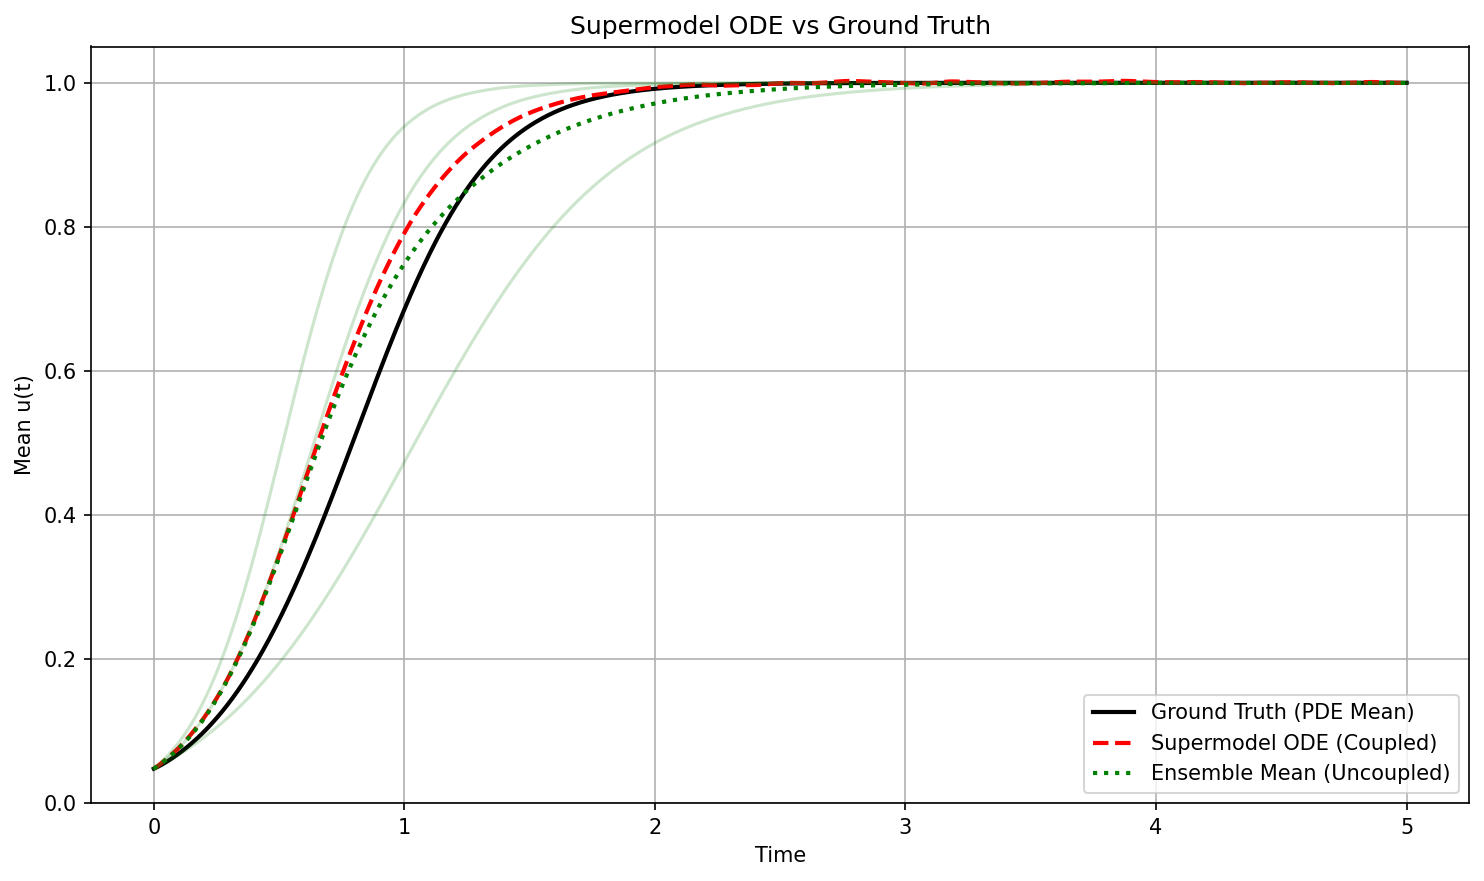
\includegraphics[width=0.8\textwidth]{../zad7/results/supermodel_ode_results.png}
  \caption{SuperModel ODE (red) vs Truth (black) vs single models (green).}
\end{figure}
\begin{itemize}
    \item Single models with perturbed parameters (p, q) deviate significantly from the truth.
    \item The coupled SuperModel reduces the error, though with a slight overshoot in the saturation phase.
    \item \textbf{RMSE Single ODE:} 0.111640 \qquad \textbf{RMSE Supermodel:} 0.045112.
\end{itemize}
\end{frame}

\begin{frame}{Results: SuperNet PINN (Improved)}
\begin{itemize}
    \item \textbf{Training (improved):} 3 PINN networks, 2000 epochs, time: 156.08s (CPU), 5\% measurement noise + Coupling Loss.
    \item \textbf{Architecture:} Each network: 5 layers $\times$ 64 neurons with residual connections (as in task 6)
    \item \textbf{Optimization:} Learning rate scheduler, gradient clipping, \textbf{warmup Coupling Loss} ($\lambda_{couple}$: 0.1 $\to$ 0.5 over 500 epochs)
    \item \textbf{Loss (last):} Total $\approx0.030$ (much better than before) - balanced convergence.
\end{itemize}
\begin{figure}
  \centering
  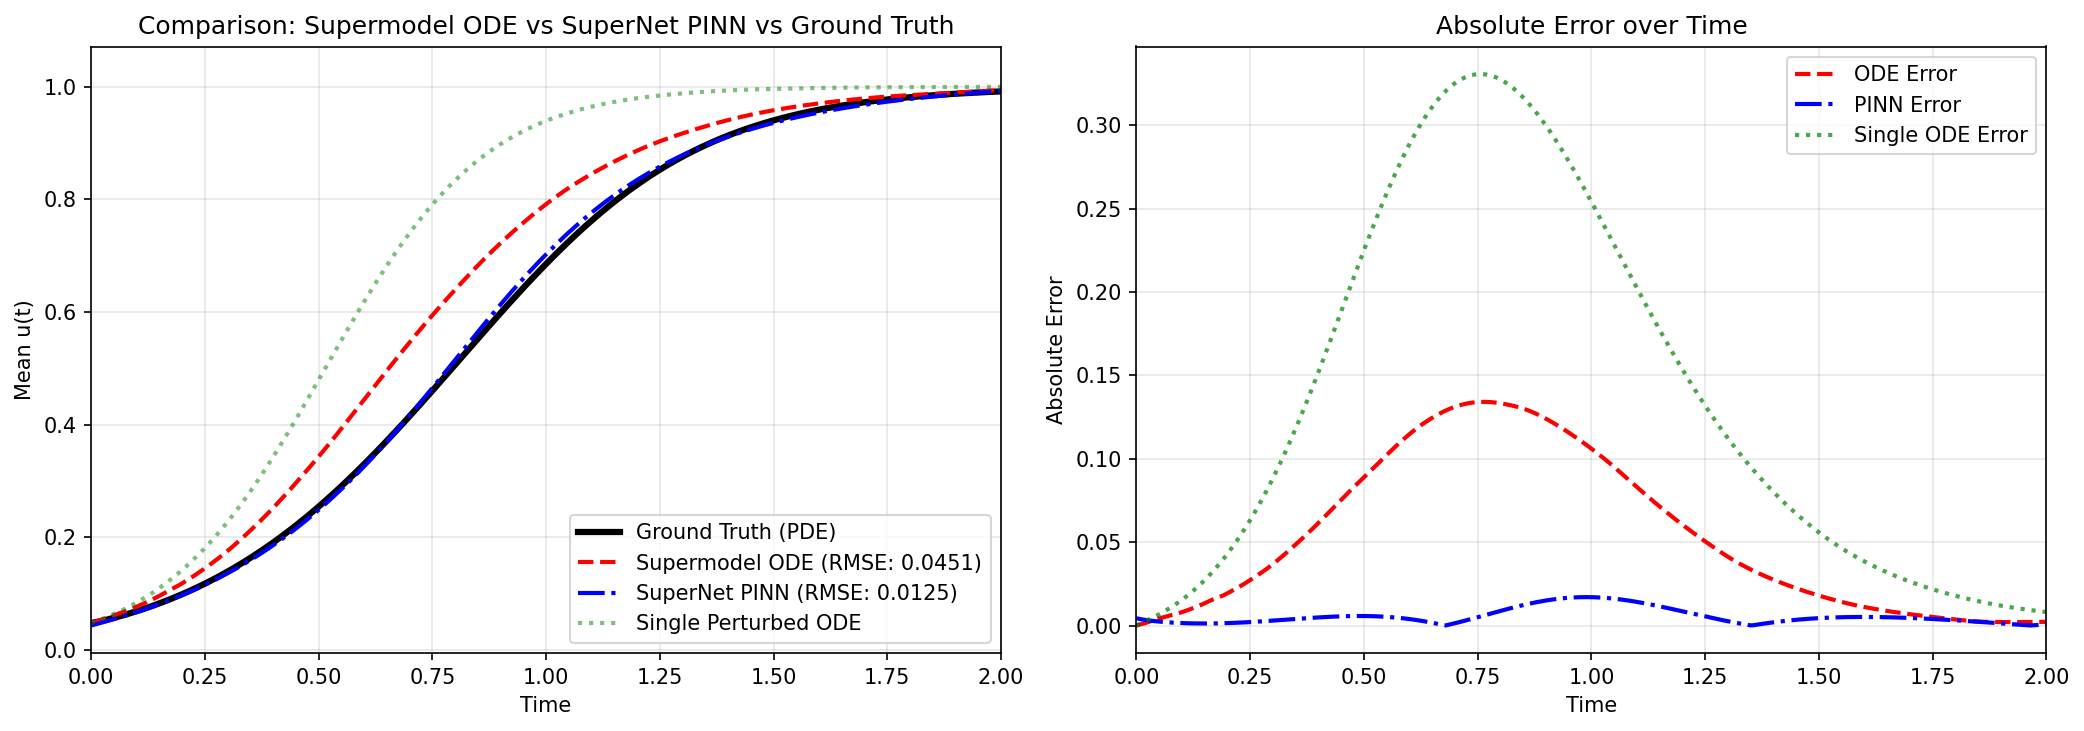
\includegraphics[width=0.8\textwidth]{../zad7/results/supermodel_vs_supernet_improved.png}
  \caption{Comparison: SuperNet PINN (improved, blue) vs SuperModel ODE (red) vs Truth (black).}
\end{figure}
\end{frame}

\begin{frame}{Summary and Final Conclusions (Tasks 6 and 7)}
\begin{table}
\centering
\begin{tabular}{l|cc}
\textbf{Model} & \textbf{MAE} & \textbf{RMSE} \\
\hline
\textbf{Task 6:} & & \\
  Single PINN (baseline) & 0.1855 & 0.2359 \\
  PINN (improved) & \textbf{0.0314} & \textbf{0.0612} \\
\hline
\textbf{Task 7:} & & \\
  Single Perturbed ODE & 0.0549 & 0.1116 \\
  SuperModel ODE & 0.0222 & 0.0451 \\
  SuperNet PINN (improved) & \textbf{0.0107} & \textbf{0.0125} \\
\end{tabular}
\caption{Reconstruction error comparison of the mean dynamics - baseline vs. improved models.}
\end{table}

\textbf{Key findings:}
\begin{itemize}
  \item \textbf{Task 6:} Residual architecture + physics warmup gave a 74-83\% reduction in PINN error
  \item \textbf{Task 7:} SuperNet PINN (with residual coupling and optimization) \textbf{outperforms} the SuperModel ODE (MAE: 0.0107 vs 0.0222, RMSE: 0.0125 vs 0.0451)
  \item Deep networks + residual flow + adaptive loss-component weighting $\to$ significantly better generalization and accuracy
\end{itemize}
\end{frame}

\begin{frame}{Discussion of Results and Practical Implications}
\begin{itemize}
  \item \textbf{PINN (Task 6):} With the right architecture and training strategy, a PINN can effectively combine noisy data with physical knowledge while avoiding overfitting.
  \item \textbf{SuperNet (Task 7):} The PINN ensemble approach achieves better results than the SuperModel ODE thanks to: (i) larger network capacity, (ii) flexibility in modeling interactions within the ensemble, (iii) better assimilation of physics.
  \item \textbf{Remaining challenges:} Network interpretability, costly higher-order derivative computation, the need for hyperparameter tuning.
  \item \textbf{Recommendations:} For problems with noisy data use (a) deep networks with residual connections, (b) learning rate scheduling, (c) warmup for physics weights, (d) model ensembles to reduce variance.
\end{itemize}
\end{frame}

\bibliographystyle{plain}
\bibliography{../report/bibliography}

\end{document}
